\clearpage
\bookpart{非光滑优化}{Nonsmooth Optimization}
\label{part:nonsmooth-optimization}

\BookPartGuide{%
绝对值、最大值和稀疏惩罚在某些点上没有普通梯度，而这些点恰恰常常是最优解所在的位置，所以不能把它们当作可以忽略的例外。本部分回答：梯度不存在时，用什么判别最优，又用什么推动迭代。

第~\ref{chap:nonsmooth-composite-optimization}章先用次微分推广梯度的角色，建立次梯度方法和最优性条件。若目标分成光滑部分和容易处理的非光滑部分，邻近映射可以把非光滑部分留在子问题里精确处理，由此得到邻近梯度法及其加速版本。另一条路线是改变目标：用光滑函数替代尖点，再调用光滑优化的工具，此时需要同时控制替代误差与求解误差。最后介绍用上界或支撑信息构造代理模型的方法。}

\chapter{非光滑优化}
\label{chap:nonsmooth-composite-optimization}

用两个特征拟合三个观测，同时希望用到的特征尽量少。一种常见的写法是在最小二乘后面加上系数绝对值的和：
\begin{equation}
 F(\bm{x})=\frac12\lVert\bm{A}\bm{x}-\bm{b}\rVert_2^2+\lambda\lVert\bm{x}\rVert_1,\qquad
 \bm{A}=\begin{pmatrix}1&1\\1&0\\0&1\end{pmatrix},\quad
 \bm{b}=\begin{pmatrix}3\\2\\-1\end{pmatrix},\quad
 \lambda=1.
 \label{eq:ns-lasso-example}
\end{equation}
后面会算出它的解是$\bm{x}^\star=(2,0)$：第二个系数恰好等于零。这个零不是巧合，绝对值项的作用正是把解压到坐标轴上。

麻烦也在这里。第~\ref{chap:smooth-foundations}章和第~\ref{chap:first-order-methods}章的方法都要读梯度，$\lvert x_2\rvert$在$x_2=0$处却没有导数。在解的附近，目标的等高线带着尖角，“梯度为零”这个判据根本无从写起。不可微的点恰好是解所在的点，这是非光滑优化的特点，不能靠“几乎处处可微”绕过去。

本章先回答怎样判断最优：第~\ref{sec:ns-subdifferential}节用支撑直线的斜率代替导数。有了这个工具，最直接的做法是把梯度换成次梯度，第~\ref{sec:ns-subgradient}节会看到这样做每步不一定下降，但有限步后的目标差仍可控制，代价是速度很慢。

慢的根源在于把尖点的结构丢掉了。后面三节用三种不同的办法把结构用回来。第~\ref{sec:ns-proximal}节和第~\ref{sec:ns-composite}节把难求导的部分原样保留在一个带二次距离项的小问题里，当这个小问题有闭式解时，就得到ISTA和FISTA。第~\ref{sec:ns-smoothing}节把尖点磨圆，换成一个光滑的目标，再调用光滑优化的方法，这时要同时算清磨圆带来的偏差和求解的误差。第~\ref{sec:ns-surrogate}节在每一轮构造一个容易求解的模型，模型可以是上界，也可以是由次梯度拼成的下界，两者的用法不同。

全章反复使用三个小例子，除式~\eqref{eq:ns-lasso-example}外，还有一维的三段折线和二维的菱形目标：
\begin{equation}
 f(x)=\max\Bigl\{-x,\ \frac{x}{2},\ 2x-3\Bigr\},\qquad
 f(\bm{x})=\lvert x_1\rvert+2\lvert x_2\rvert.
 \label{eq:ns-running-examples}
\end{equation}
两者的最优解都是原点，最优值都是$0$，下文分别称为三段折线和菱形目标。

\section{次微分}
\label{sec:ns-subdifferential}

函数在尖点没有导数，“导数为零”也就无从谈起。于是要问：在不可微的点，用什么量代替梯度，才能判断这个点是否最优？

\paragraph{尖点上的斜率}
先看$f(x)=\lvert x\rvert$。在$x\neq0$处，唯一的切线同时也是函数图像下方的一条支撑线。在$x=0$处没有切线，但有许多直线穿过原点且整条都不高于函数图像，也就是斜率$s$满足
\[
 \lvert y\rvert\geq s\,y\qquad\text{对所有}\ y.
\]

这个不等式对$s\in[-1,1]$成立，超出这个范围就会在某一侧穿到函数上方。图~\ref{fig:ns-support-lines}(a)画出了其中五条。

\begin{BookInlineFigure}
  \centering
  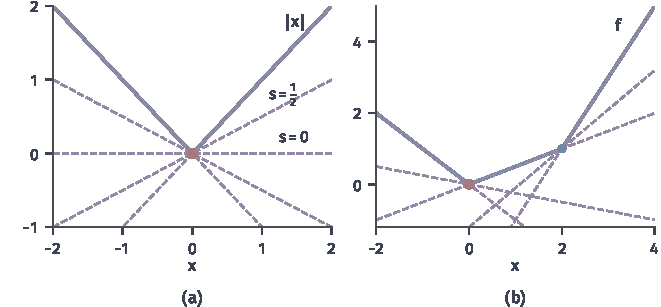
\includegraphics[width=112mm]{figures/05-optimization/03-nonsmooth-optimization/matplotlib/ns-support-lines/figure.pdf}
  \caption{尖点上的支撑直线。蓝线是函数，紫色虚线是不高于函数图像且在该点接触的直线，红点是最优解。(a)$\lvert x\rvert$在原点有斜率从$-1$到$1$的一整族支撑线，斜率$s=0$的水平线也在其中。(b)三段折线在$x=0$处的支撑斜率取遍$[-1,\tfrac12]$，在$x=2$处取遍$[\tfrac12,2]$，图中各画出几条。}
  \label{fig:ns-support-lines}
\end{BookInlineFigure}

可以把这些直线想成垫在碗底的一块木板。光滑的碗底只有一种放法，木板的倾角就是导数。碗底是尖的，木板可以在一定范围内摇摆，每个摆得开的倾角都是一条合格的支撑线。这个图景有一个边界：木板必须托住整个函数，不只是局部，所以下面的定义只适合凸函数。

\begin{definition}[次梯度与次微分]
\label{def:ns-subgradient}
设$f:\mathbb{R}^n\to\mathbb{R}\cup\{+\infty\}$是适当的凸函数，$\bm{x}\in\operatorname{dom}f$。若向量$\bm{g}\in\mathbb{R}^n$满足
\begin{equation}
 f(\bm{y})\geq f(\bm{x})+\langle\bm{g},\bm{y}-\bm{x}\rangle\qquad\text{对所有}\ \bm{y}\in\mathbb{R}^n,
 \label{eq:ns-subgradient}
\end{equation}
就称$\bm{g}$是$f$在$\bm{x}$处的\term{次梯度}（subgradient）。全体次梯度组成的集合
\begin{equation}
 \partial f(\bm{x})=\bigl\{\bm{g}:\ \bm{g}\ \text{满足式~\eqref{eq:ns-subgradient}}\bigr\}
 \label{eq:ns-subdifferential}
\end{equation}
称为$f$在$\bm{x}$处的\term{次微分}（subdifferential）。对$\bm{x}\notin\operatorname{dom}f$，规定$\partial f(\bm{x})=\varnothing$。
\end{definition}

式~\eqref{eq:ns-subgradient}的量词是“对所有$\bm{y}$”，这是全局信息。一元时它说的正是支撑线。多元时，右端是一个仿射函数的图像，也就是一张支撑超平面，它把函数的\term{上图}（epigraph）$\{(\bm{y},v):v\geq f(\bm{y})\}$整个留在上方。

次梯度与第~\ref{chap:optimization}章的梯度不是两种东西，可微点上它们重合。下面的定理同时说明，次微分什么时候确实存在。

\begin{theorem}[次微分的基本性质]
\label{thm:ns-subdiff-basic}
设$f$是适当的凸函数。
\begin{enumerate}
 \item $\partial f(\bm{x})$总是闭凸集（可能为空）。
 \item 若$f$在$\bm{x}\in\operatorname{int}\operatorname{dom}f$处可微，则$\partial f(\bm{x})=\{\nabla f(\bm{x})\}$。
 \item 若$\bm{x}\in\operatorname{int}\operatorname{dom}f$，则$\partial f(\bm{x})$非空且有界。
\end{enumerate}
\end{theorem}

\begin{proof}
第一条：每个固定的$\bm{y}$，把式~\eqref{eq:ns-subgradient}看成$\bm{g}$的条件，都给出一个闭半空间。$\partial f(\bm{x})$是这些闭半空间的交，所以是闭凸集。

第二条：设$\bm{g}\in\partial f(\bm{x})$，$\bm{d}$是任意方向。在式~\eqref{eq:ns-subgradient}中取$\bm{y}=\bm{x}+s\bm{d}$，$s>0$，得到
\[
 \frac{f(\bm{x}+s\bm{d})-f(\bm{x})}{s}\geq\langle\bm{g},\bm{d}\rangle.
\]

令$s\to0^+$，左端趋于$\langle\nabla f(\bm{x}),\bm{d}\rangle$，于是
\[
 \langle\nabla f(\bm{x})-\bm{g},\bm{d}\rangle\geq0\qquad\text{对所有}\ \bm{d}.
\]
取$\bm{d}=\bm{g}-\nabla f(\bm{x})$，只能有$\bm{g}=\nabla f(\bm{x})$。反过来，第~\ref{chap:optimization}章已经说明，凸函数的切平面是全局下界，所以$\nabla f(\bm{x})\in\partial f(\bm{x})$。

第三条的有界性：取$r>0$使闭球$\{\bm{y}:\lVert\bm{y}-\bm{x}\rVert_2\leq r\}$在$\operatorname{dom}f$内，凸函数在这个紧集上有上界$B$（把球放进一个小单纯形，函数值不超过顶点值的最大值）。对非零的$\bm{g}\in\partial f(\bm{x})$，取$\bm{y}=\bm{x}+r\bm{g}/\lVert\bm{g}\rVert_2$，由式~\eqref{eq:ns-subgradient}，
\[
 B\geq f(\bm{y})\geq f(\bm{x})+r\lVert\bm{g}\rVert_2.
\]
所以$\lVert\bm{g}\rVert_2\leq(B-f(\bm{x}))/r$。

第三条的非空性要用支撑超平面定理：上图是凸集，$(\bm{x},f(\bm{x}))$在它的边界上，过这一点存在一张支撑超平面。还需排除竖直的超平面，这一步由$\bm{x}$是内点保证。
\end{proof}

第三条非空性的详细论证可查阅\scite{rockafellar1970convex}。

边界点上次微分可以是空的。图~\ref{fig:ns-no-support}(a)的函数$f(x)=-\sqrt{x}$（$x\geq0$，其余为$+\infty$）是凸的，在$x=0$处切线竖直。任何有限斜率$s$的直线$sy$，在$y$足够小时都高于$-\sqrt{y}$，因为
\[
 -\sqrt{y}\geq s\,y\quad\Longleftrightarrow\quad\sqrt{y}\,(1+s\sqrt{y})\leq0,
\]
当$y\to0^+$时左端为正。所以$\partial f(0)=\varnothing$。第三条要求内点，正是为了排除这种情形。

\begin{BookInlineFigure}
  \centering
  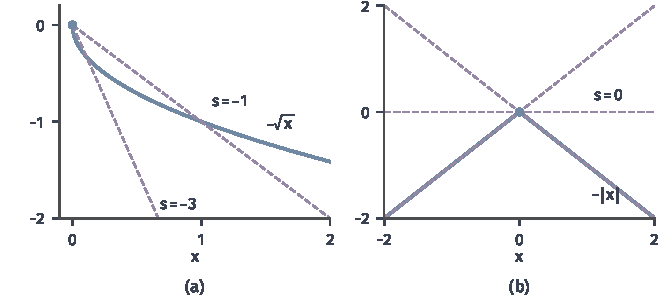
\includegraphics[width=112mm]{figures/05-optimization/03-nonsmooth-optimization/matplotlib/ns-no-support/figure.pdf}
  \caption{支撑线不存在的两种情形。(a)凸函数$-\sqrt{x}$在定义域端点切线竖直，紫色虚线（斜率$-1$和$-3$）在原点右侧贴近处都高出函数图像，所以次微分为空。(b)非凸函数$-\lvert x\rvert$的尖点朝上，任何穿过原点的直线都有一部分高于函数，按全局定义没有次梯度。}
  \label{fig:ns-no-support}
\end{BookInlineFigure}

\paragraph{几个计算}
绝对值的次微分由上面的讨论得到：
\begin{equation}
 \partial\lvert x\rvert=\begin{cases}\{\operatorname{sign}(x)\},&x\neq0,\\ [-1,1],&x=0.\end{cases}
 \label{eq:ns-abs-subdiff}
\end{equation}

坐标可分的函数$\sum_ic_i\lvert x_i\rvert$（$c_i>0$）的次微分是各坐标次微分的乘积。这是因为支撑不等式可以逐坐标相加，反过来只让一个坐标变化，就把每个坐标的不等式分离出来。

以菱形目标$f(\bm{x})=\lvert x_1\rvert+2\lvert x_2\rvert$为例，三个代表点的结果是
\[
 \partial f(0,0)=[-1,1]\times[-2,2],\quad
 \partial f(1,0)=\{1\}\times[-2,2],\quad
 \partial f(\tfrac12,\tfrac12)=\{(1,2)\}.
\]

图~\ref{fig:ns-diamond-subdiff}把点放在左边的$\bm{x}$平面，把次微分放在右边的斜率平面。越是“尖”的点，次微分越大：顶点处是长方形，棱上是线段，光滑的面内缩成一点。

\begin{BookInlineFigure}
  \centering
  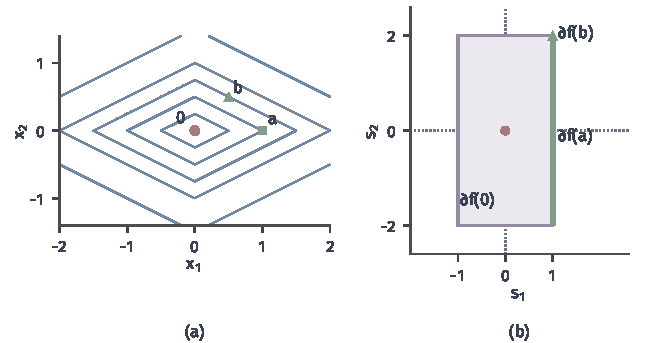
\includegraphics[width=112mm]{figures/05-optimization/03-nonsmooth-optimization/matplotlib/ns-diamond-subdiff/figure.pdf}
  \caption{菱形目标的次微分。(a)蓝线是$\lvert x_1\rvert+2\lvert x_2\rvert$的等高线，红点是最优解，$a=(1,0)$在棱上，$b=(\tfrac12,\tfrac12)$在光滑部分。(b)斜率平面：紫色长方形是原点的次微分，绿色粗线段是$a$处的次微分，绿色三角是$b$处的梯度。只有长方形包含$\bm{0}$（红点）。}
  \label{fig:ns-diamond-subdiff}
\end{BookInlineFigure}

有限个函数取最大值是尖点的另一个来源。最大值的尖点出现在分支交替的地方，这时次微分由活跃分支的梯度张成。把有限个向量的全部凸组合$\sum_i\theta_i\bm{g}_i$（$\theta_i\geq0$，$\sum_i\theta_i=1$）组成的集合称为它们的\term{凸包}（convex hull），记作$\operatorname{conv}$。

\begin{theorem}[有限最大值的次微分]
\label{thm:ns-max-subdiff}
设$f_1,\ldots,f_m:\mathbb{R}^n\to\mathbb{R}$都是可微的凸函数，$f=\max_if_i$，$I(\bm{x})=\{i:f_i(\bm{x})=f(\bm{x})\}$是活跃下标集。则
\begin{equation}
 \partial f(\bm{x})=\operatorname{conv}\bigl\{\nabla f_i(\bm{x}):\ i\in I(\bm{x})\bigr\}.
 \label{eq:ns-max-subdiff}
\end{equation}
\end{theorem}

\begin{proof}
记右端为$\bm{K}$。先证$\bm{K}\subseteq\partial f(\bm{x})$。对活跃的$i$和任意$\bm{y}$，
\[
 f(\bm{y})\geq f_i(\bm{y})\geq f_i(\bm{x})+\langle\nabla f_i(\bm{x}),\bm{y}-\bm{x}\rangle=f(\bm{x})+\langle\nabla f_i(\bm{x}),\bm{y}-\bm{x}\rangle.
\]
把这些不等式按$\theta_i$加权相加，就得到凸组合也满足式~\eqref{eq:ns-subgradient}。

再证反向。假设$\bm{g}\in\partial f(\bm{x})$但$\bm{g}\notin\bm{K}$。$\bm{K}$是紧凸集，可以严格分离：存在方向$\bm{d}$，使
\[
 \langle\bm{g},\bm{d}\rangle>\max_{i\in I(\bm{x})}\langle\nabla f_i(\bm{x}),\bm{d}\rangle.
\]

当$s>0$足够小时，不活跃的分支仍低于活跃分支，所以
\[
 f(\bm{x}+s\bm{d})=f(\bm{x})+s\max_{i\in I(\bm{x})}\langle\nabla f_i(\bm{x}),\bm{d}\rangle+o(s).
\]

另一方面，由式~\eqref{eq:ns-subgradient}，
\[
 f(\bm{x}+s\bm{d})\geq f(\bm{x})+s\langle\bm{g},\bm{d}\rangle.
\]
两式合起来除以$s$，令$s\to0^+$，与严格不等式矛盾。
\end{proof}

用这个定理算三段折线$f(x)=\max\{-x,x/2,2x-3\}$。三个分支的斜率是$-1,\tfrac12,2$。在$x=0$处前两支活跃，在$x=2$处后两支活跃，所以
\[
 \partial f(0)=[-1,\tfrac12],\qquad\partial f(2)=[\tfrac12,2].
\]

其余点只有一支活跃，次微分是单点。图~\ref{fig:ns-subdiff-graph}(b)把$\partial f(x)$画成$x$的集值图：普通的点对应水平线段上的一个值，尖点对应一条竖直线段，整条曲线是单调上升的台阶。单调上升这件事对应一元凸函数的导数非减。

\begin{BookInlineFigure}
  \centering
  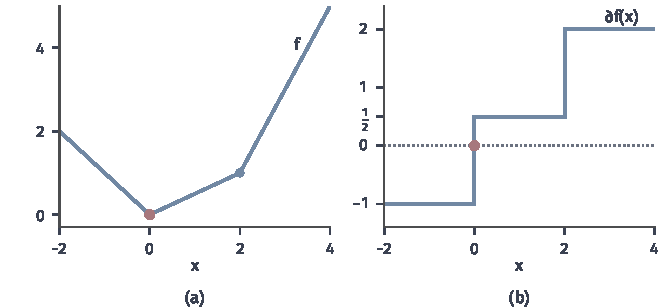
\includegraphics[width=112mm]{figures/05-optimization/03-nonsmooth-optimization/matplotlib/ns-subdiff-graph/figure.pdf}
  \caption{三段折线与它的次微分。(a)函数图像，红点是最优解。(b)次微分的集值图像，在两个折点处是竖直线段，点线是斜率为零的水平线。折线在$x=0$处的竖直线段穿过零，这就是最优性条件。}
  \label{fig:ns-subdiff-graph}
\end{BookInlineFigure}

\paragraph{最优性条件}
回到本节的问题。式~\eqref{eq:ns-subgradient}中令$\bm{g}=\bm{0}$，恰好读作“$f(\bm{y})\geq f(\bm{x})$对所有$\bm{y}$成立”。判据由此直接得到。

\begin{theorem}[凸目标的最优性条件]
\label{thm:ns-fermat}
设$f$是适当的凸函数，则
\begin{equation}
 \bm{x}^\star\in\argmin_{\bm{x}}f(\bm{x})\quad\Longleftrightarrow\quad\bm{0}\in\partial f(\bm{x}^\star).
 \label{eq:ns-fermat}
\end{equation}
\end{theorem}

\begin{proof}
由次梯度定义~\eqref{eq:ns-subgradient}，$\bm{0}\in\partial f(\bm{x}^\star)$与“对所有$\bm{y}$，$f(\bm{y})\geq f(\bm{x}^\star)$”是同一句话。
\end{proof}

这个判据比第~\ref{chap:optimization}章的一阶条件走得更远：它是充要的，而且结论是全局的，因为全局性已经写在定义里了。图~\ref{fig:ns-subdiff-graph}上读这个判据，就是找集值图穿过零线的地方。三段折线在$x=0$处$0\in[-1,\tfrac12]$，是最优解；在$x=2$处$0\notin[\tfrac12,2]$，不是。图~\ref{fig:ns-diamond-subdiff}(b)中，只有长方形包含原点。

\paragraph{和与复合的规则}
复杂的目标由简单的项拼成，希望次微分也能逐项计算。部分结论无条件成立，另一部分需要一个正则条件。下面用$\operatorname{ri}$表示\term{相对内部}（relative interior）：在集合自身张成的仿射子空间内的内点。若$\operatorname{dom}f$有内点，$\operatorname{ri}\operatorname{dom}f$就是内部。

\begin{theorem}[和与仿射复合]
\label{thm:ns-sum-rule}
设$f_1,f_2,f$是适当的凸函数，$\bm{A}\in\mathbb{R}^{p\times n}$，$\bm{c}\in\mathbb{R}^p$。对任意$\bm{x}$，
\begin{gather}
 \partial f_1(\bm{x})+\partial f_2(\bm{x})\subseteq\partial(f_1+f_2)(\bm{x}),\label{eq:ns-sum-inclusion}\\
 \bm{A}^\top\partial f(\bm{A}\bm{x}+\bm{c})\subseteq\partial\bigl(f(\bm{A}\,\cdot+\bm{c})\bigr)(\bm{x}).\label{eq:ns-affine-inclusion}
\end{gather}
若$\operatorname{ri}\operatorname{dom}f_1\cap\operatorname{ri}\operatorname{dom}f_2\neq\varnothing$，式~\eqref{eq:ns-sum-inclusion}取等号。若$\bm{A}$的值域经平移后与$\operatorname{ri}\operatorname{dom}f$相交，即存在$\bm{x}_0$使$\bm{A}\bm{x}_0+\bm{c}\in\operatorname{ri}\operatorname{dom}f$，式~\eqref{eq:ns-affine-inclusion}取等号。
\end{theorem}

\begin{proof}
两个包含关系只用定义。若$\bm{g}_i\in\partial f_i(\bm{x})$，把两条支撑不等式相加，就得到$\bm{g}_1+\bm{g}_2$是$f_1+f_2$的次梯度。若$\bm{g}\in\partial f(\bm{A}\bm{x}+\bm{c})$，对任意$\bm{y}$，
\[
 \begin{aligned}
 f(\bm{A}\bm{y}+\bm{c})&\geq f(\bm{A}\bm{x}+\bm{c})+\langle\bm{g},\bm{A}(\bm{y}-\bm{x})\rangle\\
 &=f(\bm{A}\bm{x}+\bm{c})+\langle\bm{A}^\top\bm{g},\bm{y}-\bm{x}\rangle.
 \end{aligned}
\]

反向的包含要由分离定理构造出分解，正则条件正是分离定理不退化所需要的，篇幅较长，可查阅凸分析的专著。
\end{proof}

下面的两个反例说明这些条件不能去掉。

先看和的反例。取$f_1(x)=-\sqrt{x}$（$x\geq0$，其余为$+\infty$），$f_2$是$(-\infty,0]$的约束指标函数。两者的有效定义域只在$0$处相交，相对内部$(0,\infty)$与$(-\infty,0)$不相交，条件不满足。$f_1+f_2$只在$0$处有限，所以
\[
 \partial(f_1+f_2)(0)=\mathbb{R},\qquad\partial f_1(0)+\partial f_2(0)=\varnothing.
\]
左边是整条实线，右边什么都没有，因为前面已经算出$\partial f_1(0)=\varnothing$。

再看复合的反例。取$f(u_1,u_2)=-\sqrt{u_2}$（$u_2\geq0$，其余为$+\infty$），$\bm{A}x=(x,0)$。值域是直线$u_2=0$，只碰到$\operatorname{dom}f$的边界。复合函数恒等于$0$，次微分是$\{0\}$，而$\partial f(x,0)=\varnothing$，等式同样失败。

实际中最常见的情形，至少有一项在全空间有限，比如$\lvert x\rvert$、$\lVert\bm{x}\rVert_1$和光滑项，正则条件自动成立。约束指标函数加有限函数也是如此，只要约束集非空。

外层是一元函数的复合还有一条常用规则：设$\psi:\mathbb{R}\to\mathbb{R}$是非减的凸函数，$c:\mathbb{R}^n\to\mathbb{R}$是可微的凸函数，则$\psi\circ c$是凸函数，且
\begin{equation}
 \partial(\psi\circ c)(\bm{x})=\bigl\{s\nabla c(\bm{x}):\ s\in\partial\psi(c(\bm{x}))\bigr\}.
 \label{eq:ns-monotone-chain}
\end{equation}

式~\eqref{eq:ns-monotone-chain}中“$\supseteq$”的方向可以直接验证。由$\psi$的支撑不等式和$s\geq0$（$\psi$非减保证了这一点），
\[
 \psi(c(\bm{y}))\geq\psi(c(\bm{x}))+s\bigl(c(\bm{y})-c(\bm{x})\bigr)\geq\psi(c(\bm{x}))+s\langle\nabla c(\bm{x}),\bm{y}-\bm{x}\rangle.
\]

第二步用到$s\geq0$和$c$的凸性。“$\subseteq$”的方向仍需要方向导数的论证。

例如$f(x)=\max\{0,x^2-1\}$，取$\psi=\max\{0,\cdot\}$，$c=x^2-1$。在$x=1$处，外层的次微分和内层的导数分别是
\[
 \partial\psi(0)=[0,1],\qquad c'(1)=2,
\]
于是$\partial f(1)=[0,2]$，这与函数左边斜率$0$、右边斜率$2$相符。若外层不单调，凸性本身就可能失败：$\lvert x^2-1\rvert$在$x=0$附近向下弯，式~\eqref{eq:ns-monotone-chain}不再适用。

\paragraph{贯穿例的最优性}
现在可以写出复合目标的最优性条件，并手工核验章首的问题。对
\begin{equation}
 F(\bm{x})=\frac12\lVert\bm{A}\bm{x}-\bm{b}\rVert_2^2+\lambda\lVert\bm{x}\rVert_1,\qquad\lambda>0,
 \label{eq:ns-lasso}
\end{equation}
这个问题常称为\term{Lasso}（least absolute shrinkage and selection operator）。两项都在全空间有限，和规则取等号。记$\bm{w}=\bm{A}^\top(\bm{A}\bm{x}-\bm{b})$，则$\bm{x}$最优当且仅当对每个坐标
\begin{equation}
 w_i=-\lambda\operatorname{sign}(x_i)\quad(x_i\neq0),\qquad\lvert w_i\rvert\leq\lambda\quad(x_i=0).
 \label{eq:ns-lasso-optimality}
\end{equation}

非零坐标上光滑项的梯度被绝对值的斜率恰好抵消；零坐标上梯度只要不超过$\lambda$，绝对值在零点的那一段斜率范围足以把它吸收，这个坐标便可以留在零。这就是Lasso产生零系数的机制。

验证例~\eqref{eq:ns-lasso-example}的候选解$\bm{x}^\star=(2,0)$。先算残差和梯度：
\[
 \bm{A}\bm{x}^\star-\bm{b}=(-1,0,1),\qquad\bm{w}=\bm{A}^\top(\bm{A}\bm{x}^\star-\bm{b})=(-1,0).
\]

第一坐标$x_1=2>0$，要求$w_1=-1$，成立。第二坐标$x_2=0$，要求$\lvert w_2\rvert\leq1$，成立。因此$\bm{x}^\star=(2,0)$是最优解，最优值为
\[
 F^\star=\frac12(1+0+1)+2=3.
\]

相对地，原点不是解：此处$\bm{w}=-\bm{A}^\top\bm{b}=(-5,-2)$，两个分量的绝对值都超过$1$。

约束问题也可以放进这个框架。设$\bm{C}$是非空闭凸集，$\iota_{\bm{C}}$是它的约束指标函数。按定义，$\bm{g}\in\partial\iota_{\bm{C}}(\bm{x})$（$\bm{x}\in\bm{C}$）当且仅当
\begin{equation}
 \langle\bm{g},\bm{y}-\bm{x}\rangle\leq0\qquad\text{对所有}\ \bm{y}\in\bm{C}.
 \label{eq:ns-normal-cone}
\end{equation}

满足这个不等式的向量组成$\bm{C}$在$\bm{x}$处的\term{法锥}（normal cone），记作$\bm{N}_{\bm{C}}(\bm{x})$。若$f$在全空间有限且凸，由定理~\ref{thm:ns-fermat}和和规则，$\bm{x}^\star$是约束问题的解当且仅当$\bm{0}\in\partial f(\bm{x}^\star)+\bm{N}_{\bm{C}}(\bm{x}^\star)$。例如在$[0,1]$上最小化$(x-3)^2/2$，解是边界点$x^\star=1$，此处$f'(1)=-2$，$\bm{N}(1)=[0,\infty)$，所以$0\in-2+[0,\infty)$。这个判据在第~\ref{chap:constrained-optimality}章会展开成乘子形式。

\paragraph{非凸函数的广义导数}
定义~\ref{def:ns-subgradient}依赖全局不等式，离开凸函数就不再合适。图~\ref{fig:ns-no-support}(b)的$-\lvert x\rvert$在原点按全局定义没有次梯度，但它是局部Lipschitz函数，尖点处的斜率信息是有意义的。常用的办法是只看局部，把附近可微点的梯度取极限。

对局部Lipschitz函数$f$，几乎处处可微，令$\bm{D}$为可微点集合，定义\term{Clarke次微分}（Clarke subdifferential）
\begin{equation}
 \partial_{\mathrm{C}}f(\bm{x})=\operatorname{conv}\Bigl\{\lim_{k\to\infty}\nabla f(\bm{x}^{(k)}):\ \bm{x}^{(k)}\to\bm{x},\ \bm{x}^{(k)}\in\bm{D}\Bigr\}.
 \label{eq:ns-clarke}
\end{equation}

这里的$(k)$是取极限用的序列编号。凸函数的Clarke次微分与$\partial f$相同；$f$连续可微时它就是$\{\nabla f\}$。对$-\lvert x\rvert$，$\partial_{\mathrm{C}}f(0)=[-1,1]$，包含$0$，但原点却是极大点。

可见$\bm{0}\in\partial_{\mathrm{C}}f(\bm{x})$只是局部最优的必要条件，与光滑非凸问题的“驻点”处于同一地位，不能得出全局或局部最优的结论\scite{math-clarke1990optimization}。本章其余部分遇到非凸目标时只用一种形式：$f$连续可微但可以非凸，$r$是凸函数，把$\nabla f(\bm{x})+\partial r(\bm{x})$作为$f+r$的广义次微分，$r$局部Lipschitz时它正是Clarke次微分。

\begin{BookInlineTable}
  \centering
  \small
  \begin{tabular}{@{}llll@{}}
    \toprule
    对象 & 判据 & 是否充分 & 结论范围\\
    \midrule
    光滑函数 & $\nabla f=\bm{0}$ & 否 & 局部最优的必要条件\\
    光滑凸函数 & $\nabla f=\bm{0}$ & 是 & 全局最优\\
    非光滑凸函数 & $\bm{0}\in\partial f$ & 是 & 全局最优\\
    局部Lipschitz函数 & $\bm{0}\in\partial_{\mathrm{C}}f$ & 否 & 局部最优的必要条件\\
    \bottomrule
  \end{tabular}
  \caption{不同函数类上的一阶判据。是否充分取决于凸性，与是否光滑无关。}
  \label{tab:ns-optimality}
\end{BookInlineTable}

表~\ref{tab:ns-optimality}汇总了这些判据。非光滑不会削弱判据的强度，凸性才决定“驻点”能否等于最优解。

\section{次梯度方法}
\label{sec:ns-subgradient}

有了次梯度，最直接的算法是把梯度下降里的梯度换掉。接下来要弄清：这样换了之后，每一步还是不是在下山？如果不是，靠什么保证有限步之后的目标差可以控制？

\paragraph{主要思想}
设$f:\mathbb{R}^n\to\mathbb{R}$是凸函数，每次可以读取一个函数值和一个次梯度。这种只给函数值和次梯度的读取方式常称为黑箱。\term{次梯度法}（subgradient method）的迭代是
\begin{equation}
 \bm{x}^{(t+1)}=\bm{x}^{(t)}-\alpha^{(t)}\bm{g}^{(t)},\qquad\bm{g}^{(t)}\in\partial f(\bm{x}^{(t)}).
 \label{eq:ns-subgradient-update}
\end{equation}

这里$\bm{g}^{(t)}$的记号沿用了梯度的缩写，表示读到的那一个次梯度。

先看第一个差别：$-\bm{g}^{(t)}$不一定是下降方向。取菱形目标$f(\bm{x})=\lvert x_1\rvert+2\lvert x_2\rvert$，当前点$\bm{x}=(1,0)$，$f(\bm{x})=1$。由上节的计算，$\bm{g}=(1,2)$是一个次梯度。沿$-\bm{g}$走$\alpha$：
\[
 \bm{x}^{+}=(1-\alpha,\,-2\alpha),\qquad f(\bm{x}^{+})=1-\alpha+4\alpha=1+3\alpha.
\]

无论$\alpha>0$多小，目标都上升。第二分量离开零点付出的代价$4\alpha$超过了第一分量的收益。第~\ref{chap:smooth-foundations}章的下降引理在这里完全不成立，线搜索也无从进行：沿这个方向根本没有更低的点。

但走这一步并不是白走。到最优解$\bm{x}^\star=\bm{0}$的距离的平方变成
\[
 (1-\alpha)^2+4\alpha^2=1-2\alpha+5\alpha^2,
\]
当$\alpha<\tfrac25$时比$1$小。目标上升了，到解的距离却缩短了，图~\ref{fig:ns-not-descent}画出了这个现象。

\begin{BookInlineFigure}
  \centering
  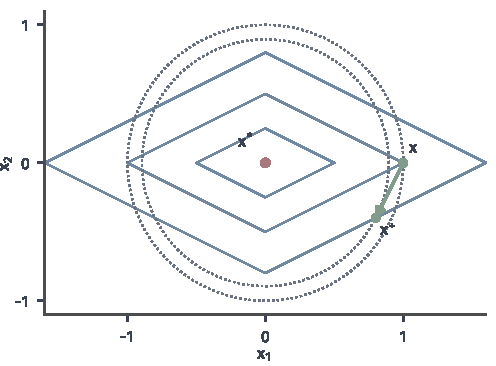
\includegraphics[width=84mm]{figures/05-optimization/03-nonsmooth-optimization/matplotlib/ns-not-descent/figure.pdf}
  \caption{次梯度步不是下降步。蓝线是菱形目标的等高线，由内到外对应$f=0.5,1,1.6$。从$\bm{x}=(1,0)$沿$-\bm{g}=-(1,2)$走$\alpha=0.2$到$\bm{x}^{+}=(0.8,-0.4)$，点越过了$f=1$的等高线，目标升到$1.6$。两个灰色点线圆以$\bm{x}^\star$（红点）为心，新点在内圆上，到解的距离从$1$降到约$0.894$。}
  \label{fig:ns-not-descent}
\end{BookInlineFigure}

原因在支撑不等式~\eqref{eq:ns-subgradient}。取$\bm{y}=\bm{x}^\star$并移项，得到
\begin{equation}
 \langle\bm{g}^{(t)},\bm{x}^{(t)}-\bm{x}^\star\rangle\geq f(\bm{x}^{(t)})-f^\star\geq0.
 \label{eq:ns-subgradient-angle}
\end{equation}

所以$-\bm{g}^{(t)}$与“指向解的方向”$\bm{x}^\star-\bm{x}^{(t)}$夹角不超过直角，目标差越大，这个内积越大。次梯度不保证等高线向内，只保证指向解的那一侧。下面的分析就用距离而不是目标值作为进展的度量。

\paragraph{计算过程}
用菱形目标$f(\bm{x})=\lvert x_1\rvert+2\lvert x_2\rvert$作例子。

\needspace{6\baselineskip}
\paragraph{变量}
\begin{itemize}
 \item $\bm{x}^{(t)}\in\mathbb{R}^n$：当前点；例中$n=2$。
 \item $\bm{g}^{(t)}$：读到的一个次梯度；例中约定把$\operatorname{sign}(0)$取成$+1$，即$\bm{g}=(\pm1,\pm2)$，这样$G=\sqrt5$。
 \item $\alpha^{(t)}$：步长；例中先用固定的$\alpha=0.3$。
 \item $f_{\mathrm{best}}$与$\bm{x}_{\mathrm{best}}$：目前最好的值和点。
\end{itemize}

\paragraph{初始化}
选起点$\bm{x}^{(0)}$，令$f_{\mathrm{best}}=f(\bm{x}^{(0)})$。例中$\bm{x}^{(0)}=(1,1)$，$f_{\mathrm{best}}=3$，到解的距离$R=\sqrt2$。

\needspace{6\baselineskip}
\paragraph{每轮更新}
\begin{enumerate}
 \item 读取$\bm{g}^{(t)}\in\partial f(\bm{x}^{(t)})$。例中第一轮$\bm{g}^{(0)}=(1,2)$。
 \item 由式~\eqref{eq:ns-subgradient-update}计算新点。例中第一轮
 \[
  \bm{x}^{(1)}=(1,1)-0.3\,(1,2)=(0.7,0.4).
 \]
 \item 计算$f(\bm{x}^{(t+1)})$，若比$f_{\mathrm{best}}$小就更新。例中$f(\bm{x}^{(1)})=1.5$，$f_{\mathrm{best}}=1.5$。
\end{enumerate}

后续各轮的结果如下，$\bm{g}^{(t)}$按当前点的符号取得：
\[
 \begin{aligned}
 \bm{x}^{(2)}&=(0.7,0.4)-0.3\,(1,2)=(0.4,-0.2), & f&=0.8,\\
 \bm{x}^{(3)}&=(0.4,-0.2)-0.3\,(1,-2)=(0.1,0.4), & f&=0.9,\\
 \bm{x}^{(4)}&=(0.1,0.4)-0.3\,(1,2)=(-0.2,-0.2), & f&=0.6,\\
 \bm{x}^{(5)}&=(-0.2,-0.2)-0.3\,(-1,-2)=(0.1,0.4), & f&=0.9.
 \end{aligned}
\]

第三轮目标从$0.8$升到$0.9$，第五轮回到了$\bm{x}^{(3)}$，此后在$(0.1,0.4)$和$(-0.2,-0.2)$之间循环。这里没有收敛，$f_{\mathrm{best}}$停在$0.6$。迭代到预定的步数$T$结束，或在已知下界时目标差足够小时结束。最终得到的不是最后一个点，而是$\bm{x}_{\mathrm{best}}=(-0.2,-0.2)$。 图~\ref{fig:ns-subgrad-cycle}画出了路径与目标值。

\begin{BookInlineFigure}
  \centering
  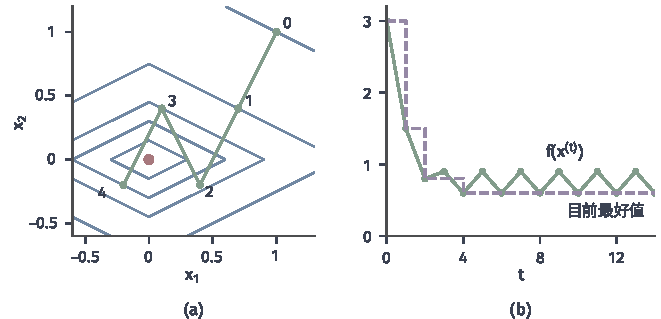
\includegraphics[width=112mm]{figures/05-optimization/03-nonsmooth-optimization/matplotlib/ns-subgrad-cycle/figure.pdf}
  \caption{固定步长$\alpha=0.3$的次梯度法。(a)菱形目标的等高线上前$5$步的路径（绿色），数字是迭代编号，最后两点形成循环。(b)绿线是目标值$f(\bm{x}^{(t)})$，反复升降；紫色虚线是目前最好值，在$0.6$处不再改善。}
  \label{fig:ns-subgrad-cycle}
\end{BookInlineFigure}

\paragraph{距离的递推}
把更新代入距离的平方并展开：
\[
 \lVert\bm{x}^{(t+1)}-\bm{x}^\star\rVert_2^2
 =\lVert\bm{x}^{(t)}-\bm{x}^\star\rVert_2^2
 -2\alpha^{(t)}\langle\bm{g}^{(t)},\bm{x}^{(t)}-\bm{x}^\star\rangle
 +(\alpha^{(t)})^2\lVert\bm{g}^{(t)}\rVert_2^2.
\]

由式~\eqref{eq:ns-subgradient-angle}替换中间一项，得到
\begin{equation}
 \lVert\bm{x}^{(t+1)}-\bm{x}^\star\rVert_2^2
 \leq\lVert\bm{x}^{(t)}-\bm{x}^\star\rVert_2^2
 -2\alpha^{(t)}\bigl(f(\bm{x}^{(t)})-f^\star\bigr)
 +(\alpha^{(t)})^2\lVert\bm{g}^{(t)}\rVert_2^2.
 \label{eq:ns-distance-recursion}
\end{equation}

式~\eqref{eq:ns-distance-recursion}中，目标差是“推进”，步长平方乘次梯度范数是“偏离”。步长小的时候偏离是二阶量，推进是一阶量，所以只要目标差还不小，距离就会缩短。目标差趋近于零时偏离占上风，迭代在解附近抖动，这决定了步长必须逐渐减小。

\begin{theorem}[次梯度法的目标差界]
\label{thm:ns-subgradient-rate}
设$f:\mathbb{R}^n\to\mathbb{R}$是凸函数，最优解$\bm{x}^\star$存在，所有读到的次梯度满足$\lVert\bm{g}^{(t)}\rVert_2\leq G$，$\lVert\bm{x}^{(0)}-\bm{x}^\star\rVert_2\leq R$。按式~\eqref{eq:ns-subgradient-update}迭代$T$步，记
\begin{equation}
 \bar{\bm{x}}^{(T)}=\frac{\sum_{t=0}^{T-1}\alpha^{(t)}\bm{x}^{(t)}}{\sum_{t=0}^{T-1}\alpha^{(t)}},\qquad
 f_{\mathrm{best}}^{(T)}=\min_{0\leq t<T}f(\bm{x}^{(t)}),
 \label{eq:ns-subgradient-outputs}
\end{equation}
则两者都满足
\begin{equation}
 \max\bigl\{f(\bar{\bm{x}}^{(T)}),\,f_{\mathrm{best}}^{(T)}\bigr\}-f^\star
 \leq\frac{R^2+G^2\sum_{t=0}^{T-1}(\alpha^{(t)})^2}{2\sum_{t=0}^{T-1}\alpha^{(t)}}.
 \label{eq:ns-subgradient-bound}
\end{equation}
特别地，预先确定$T$并取固定步长$\alpha^{(t)}=R/(G\sqrt{T})$时，上界为
\begin{equation}
 \frac{RG}{\sqrt{T}}.
 \label{eq:ns-subgradient-rate}
\end{equation}
\end{theorem}

\begin{proof}
把式~\eqref{eq:ns-distance-recursion}对$t=0,\ldots,T-1$相加，左右的距离项错项相消，只剩首尾：
\[
 \lVert\bm{x}^{(T)}-\bm{x}^\star\rVert_2^2\leq R^2-2\sum_{t=0}^{T-1}\alpha^{(t)}\bigl(f(\bm{x}^{(t)})-f^\star\bigr)+G^2\sum_{t=0}^{T-1}(\alpha^{(t)})^2.
\]

左端非负，移项后得到
\[
 2\sum_{t=0}^{T-1}\alpha^{(t)}\bigl(f(\bm{x}^{(t)})-f^\star\bigr)\leq R^2+G^2\sum_{t=0}^{T-1}(\alpha^{(t)})^2.
\]

最好值的目标差不超过各项目标差的$\alpha^{(t)}$加权平均。平均点由Jensen不等式（凸函数在加权平均点的值不超过函数值的同一加权平均，这由凸函数的定义对权重个数归纳得到）也满足
\[
 f(\bar{\bm{x}}^{(T)})-f^\star\leq\frac{\sum_t\alpha^{(t)}\bigl(f(\bm{x}^{(t)})-f^\star\bigr)}{\sum_t\alpha^{(t)}}.
\]
两者除以$2\sum_t\alpha^{(t)}$，就是式~\eqref{eq:ns-subgradient-bound}。

取$\alpha^{(t)}=\alpha$时，右端是$(R^2+TG^2\alpha^2)/(2T\alpha)$，关于$\alpha$在$\alpha=R/(G\sqrt{T})$处最小，代入即得式~\eqref{eq:ns-subgradient-rate}。
\end{proof}

定理的条件都用上了。凸性给出式~\eqref{eq:ns-subgradient-angle}；次梯度有界使偏离项可控，Lipschitz连续的函数自动满足这一条，常数$G$就是Lipschitz常数；最优解存在，$R$才有意义。结论说的是平均点或最好点，最后一点$\bm{x}^{(T)}$不在其中。

回到上面的小例子，式~\eqref{eq:ns-subgradient-bound}对$f_{\mathrm{best}}$的预言是$T=5$时不超过
\[
 \frac{2+5\cdot5\cdot0.09}{2\cdot5\cdot0.3}=\frac{4.25}{3}\approx1.417,
\]
实际的$f_{\mathrm{best}}=0.6$。当$T\to\infty$时，这个界趋于$G^2\alpha/2=0.75$，固定步长的上界也只能给到一个邻域。

\paragraph{步长规则}
式~\eqref{eq:ns-subgradient-bound}告诉我们要什么：分子增长比分母慢，这需要$\sum_t\alpha^{(t)}=\infty$，同时$\alpha^{(t)}\to0$使平方和相对于和可以忽略。满足这两条的递减步长，如$\alpha^{(t)}=c/\sqrt{t+1}$，右端趋于$0$。它们不需要预先知道$T$，代价是界多出一个对数因子。

若最优值$f^\star$已知，可以直接优化式~\eqref{eq:ns-distance-recursion}的右端。关于$\alpha^{(t)}$求最小，得到\term{Polyak步长}（Polyak step size）：
\begin{equation}
 \alpha^{(t)}=\frac{f(\bm{x}^{(t)})-f^\star}{\lVert\bm{g}^{(t)}\rVert_2^2}.
 \label{eq:ns-polyak-step}
\end{equation}

把它代回式~\eqref{eq:ns-distance-recursion}，得到每步距离的减少量：
\[
 \lVert\bm{x}^{(t+1)}-\bm{x}^\star\rVert_2^2\leq\lVert\bm{x}^{(t)}-\bm{x}^\star\rVert_2^2-\frac{(f(\bm{x}^{(t)})-f^\star)^2}{\lVert\bm{g}^{(t)}\rVert_2^2}.
\]

相加后同样得到$\min_{t<T}f(\bm{x}^{(t)})-f^\star\leq RG/\sqrt{T}$，不用事先知道$R$、$G$和$T$，但要知道$f^\star$，这在部分问题上成立，例如已知最优值为零的可行性问题。例中从$(1,0)$、$\bm{g}=(1,2)$出发，$\alpha=1/5$，点变成$(0.8,-0.4)$，就是图~\ref{fig:ns-not-descent}的那一步。

\paragraph{输出什么}
目前最好点需要每轮多算一次函数值，好处是保证单调；加权平均点不用算函数值，只需累加向量。最后一点没有上述保证。图~\ref{fig:ns-subgrad-rates}用递减步长$\alpha^{(t)}=R/(G\sqrt{t+1})$比较三者，横轴是步数，三条曲线都在上界之下，最后一点在一条带内不断跳动，目前最好点和加权平均点则是稳定的。

\begin{BookInlineFigure}
  \centering
  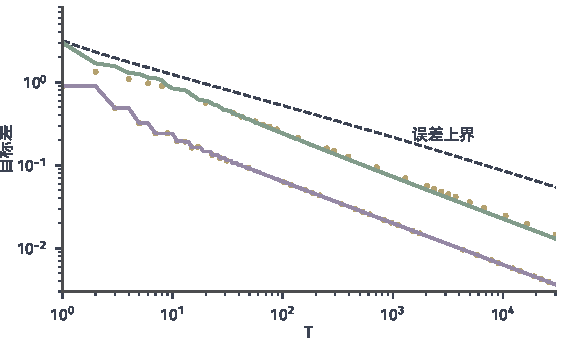
\includegraphics[width=96mm]{figures/05-optimization/03-nonsmooth-optimization/matplotlib/ns-subgrad-rates/figure.pdf}
  \caption{次梯度法的三种输出（双对数坐标）。目标是菱形目标，$\bm{x}^{(0)}=(1,1)$，步长$\alpha^{(t)}=R/(G\sqrt{t+1})$。黄点是采样的最后点目标差，它随$t$的奇偶在一条带内跳动；绿线是加权平均点；紫线是目前最好点；黑色虚线是式~\eqref{eq:ns-subgradient-bound}的上界。}
  \label{fig:ns-subgrad-rates}
\end{BookInlineFigure}

\paragraph{为什么慢，以及慢到什么程度}
要达到目标差$\varepsilon$，由式~\eqref{eq:ns-subgradient-rate}需要$T\geq R^2G^2/\varepsilon^2$步。精度提高十倍，步数增加一百倍。梯度下降在光滑凸目标上的步数是$O(1/\varepsilon)$，这里慢了一个量级。

这不是分析得不够细。只通过函数值和次梯度了解目标的方法，在维数足够大时存在最坏的函数，使任何这类方法在前若干步的目标差都不低于$RG/(2(1+\sqrt{T}))$这样的量级，所以$RG/\sqrt{T}$在黑箱模型下不能本质改进。这个下界的证明需要构造一族对抗性函数，篇幅较长，这里只用它的含义：要比$1/\sqrt{T}$更快，就不能只靠黑箱，必须用上目标的结构。

次梯度法的优势在于通用和便宜：每步只要一个次梯度，存储一个向量，不需要光滑性和邻近映射。后面几节的方法都要求多知道一些东西。

\section{邻近方法}
\label{sec:ns-proximal}

次梯度法慢，一个原因是它在尖点上只用了一个斜率，把“这里是尖的”这个信息丢了。这就需要回答：如果愿意在每一步多做一点计算，怎样把尖点的结构保留在更新里？办法是把一步更新本身写成一个小优化问题。

\subsection{邻近映射}
\label{sec:ns-prox-map}

梯度步有一个等价的写法：对光滑的$f$，$\bm{x}-\alpha\nabla f(\bm{x})$是下面二次函数的最小点，
\[
 f(\bm{x})+\langle\nabla f(\bm{x}),\bm{y}-\bm{x}\rangle+\frac{1}{2\alpha}\lVert\bm{y}-\bm{x}\rVert_2^2.
\]
这里$f$被它的一阶近似代替，再加一个二次距离项，防止走太远。如果$f$的结构足够简单，就不必做一阶近似，直接把$f$本身留在问题里。

\begin{definition}[邻近映射]
\label{def:ns-prox}
设$f:\mathbb{R}^n\to\mathbb{R}\cup\{+\infty\}$是适当、下半连续的凸函数，$\alpha>0$。输入点$\bm{x}$的\term{邻近映射}（proximal mapping）定义为
\begin{equation}
 \operatorname{prox}_{\alpha f}(\bm{x})=\argmin_{\bm{y}\in\mathbb{R}^n}\Bigl\{f(\bm{y})+\frac{1}{2\alpha}\lVert\bm{y}-\bm{x}\rVert_2^2\Bigr\}.
 \label{eq:ns-prox}
\end{equation}
\end{definition}

括号里两项在拉锯：$f$想让$\bm{y}$去函数值低的地方，距离项想让$\bm{y}$留在$\bm{x}$附近，$\alpha$决定谁的话更算数。$\alpha$很小时，结果几乎停在$\bm{x}$；$\alpha$很大时，结果接近$f$的最小点。

图~\ref{fig:ns-prox-geometry}对$f(y)=\lvert y\rvert$，$\alpha=1$画出了这种拉锯。输入$x=2$时，和函数的最小点在$p=1$处，函数值的下降抵得过距离的代价。输入$x=0.6$时，绿色曲线的最小点卡在$y=0$的尖点上：再靠近$x$的收益太小，推不动尖点。

\begin{BookInlineFigure}
  \centering
  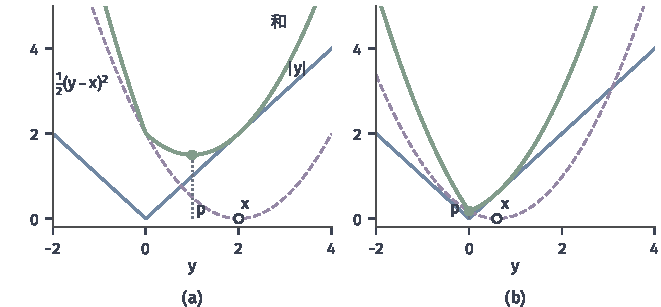
\includegraphics[width=112mm]{figures/05-optimization/03-nonsmooth-optimization/matplotlib/ns-prox-geometry/figure.pdf}
  \caption{邻近映射是一个小优化问题，$f(y)=\lvert y\rvert$，$\alpha=1$。蓝线是$f$，紫色虚线是距离项$\tfrac12(y-x)^2$，绿线是两者之和，绿点是和的最小点$p$，空心圆是输入点。(a)$x=2$，最小点$p=1$位于光滑部分。(b)$x=0.6$，最小点落在尖点$p=0$上。}
  \label{fig:ns-prox-geometry}
\end{BookInlineFigure}

定义中对$f$的要求，下面的定理逐一用到。

\begin{theorem}[邻近映射的存在、唯一与刻画]
\label{thm:ns-prox}
设$f$是适当、下半连续的凸函数，$\alpha>0$。则对每个$\bm{x}$，式~\eqref{eq:ns-prox}有唯一的最小点$\bm{p}$，并且
\begin{equation}
 \bm{p}=\operatorname{prox}_{\alpha f}(\bm{x})\quad\Longleftrightarrow\quad\frac{\bm{x}-\bm{p}}{\alpha}\in\partial f(\bm{p}).
 \label{eq:ns-prox-characterization}
\end{equation}
此外，映射是非扩张的：对任意$\bm{x},\bm{y}$，记$\bm{p}=\operatorname{prox}_{\alpha f}(\bm{x})$，$\bm{q}=\operatorname{prox}_{\alpha f}(\bm{y})$，有
\begin{equation}
 \lVert\bm{p}-\bm{q}\rVert_2^2\leq\langle\bm{p}-\bm{q},\bm{x}-\bm{y}\rangle\leq\lVert\bm{x}-\bm{y}\rVert_2\lVert\bm{p}-\bm{q}\rVert_2.
 \label{eq:ns-firm-nonexpansive}
\end{equation}
\end{theorem}

\begin{proof}
记子问题的目标为
\[
 \phi(\bm{y})=f(\bm{y})+\frac{1}{2\alpha}\lVert\bm{y}-\bm{x}\rVert_2^2.
\]

存在性。适当、下半连续的凸函数有一个仿射下界（上图是闭凸集，用分离定理得到），设$f(\bm{y})\geq a+\langle\bm{b},\bm{y}\rangle$。于是
\[
 \phi(\bm{y})\geq a+\langle\bm{b},\bm{y}\rangle+\frac{1}{2\alpha}\lVert\bm{y}-\bm{x}\rVert_2^2\to+\infty\qquad(\lVert\bm{y}\rVert_2\to\infty).
\]
所以$\phi$的下水平集有界。由第~\ref{chap:optimization}章的结果，下半连续性保证下水平集闭，下水平集紧时最小点存在。

唯一性。$\phi$是凸函数与严格凸的二次项之和，严格凸，严格凸函数至多有一个最小点。

刻画。距离项在全空间有限且可微，和规则取等号，由定理~\ref{thm:ns-fermat}，
\[
 \bm{p}\ \text{是最小点}\quad\Longleftrightarrow\quad\bm{0}\in\partial f(\bm{p})+\frac{\bm{p}-\bm{x}}{\alpha}.
\]
移项即得式~\eqref{eq:ns-prox-characterization}。

非扩张性。由式~\eqref{eq:ns-prox-characterization}，
\[
 \bm{s}=\frac{\bm{x}-\bm{p}}{\alpha}\in\partial f(\bm{p}),\qquad
 \bm{v}=\frac{\bm{y}-\bm{q}}{\alpha}\in\partial f(\bm{q}).
\]
两条支撑不等式
\[
 f(\bm{q})\geq f(\bm{p})+\langle\bm{s},\bm{q}-\bm{p}\rangle,\qquad f(\bm{p})\geq f(\bm{q})+\langle\bm{v},\bm{p}-\bm{q}\rangle
\]
相加，得到次微分的单调性$\langle\bm{s}-\bm{v},\bm{p}-\bm{q}\rangle\geq0$。代入$\bm{s},\bm{v}$的表达式并整理，
\[
 \langle(\bm{x}-\bm{y})-(\bm{p}-\bm{q}),\bm{p}-\bm{q}\rangle\geq0.
\]
这就是式~\eqref{eq:ns-firm-nonexpansive}的左半，右半是Cauchy不等式。
\end{proof}

每个条件都有用处。下半连续保证最小点取得，例如$f$在$(0,1)$内为$0$、其余为$+\infty$时，$\operatorname{dom}f$不闭，$\bm{x}=2$的最小点取不到。凸性保证唯一和式~\eqref{eq:ns-prox-characterization}。若$f=-\lvert y\rvert$，$\alpha=1$，$x=0$，$y=\pm1$都是最小点，映射不再是单值的。

\paragraph{显式步与隐式步}
把式~\eqref{eq:ns-prox-characterization}写成迭代的样子：
\begin{equation}
 \bm{x}^{+}=\bm{x}-\alpha\bm{s},\qquad\bm{s}\in\partial f(\bm{x}^{+}).
 \label{eq:ns-implicit-step}
\end{equation}

形式与次梯度步一样，差别在于斜率取在新点上。显式步先读斜率再走，隐式步要求“走到的地方的斜率正好解释这一步”。由于$\bm{x}^{+}$事先未知，这是一个隐式方程，邻近映射就是它的解。

隐式的好处看两个例子。图~\ref{fig:ns-forward-backward}(a)用$f(x)=\lvert x\rvert$，$x^{(0)}=1$，$\alpha=0.4$。次梯度步的斜率总是$\pm1$，所以点按$0.4$的步子走过零点来回跳，序列是$1,\,0.6,\,0.2,\,-0.2,\,0.2,\ldots$；邻近步在前两步相同，第三步由式~\eqref{eq:ns-implicit-step}选出$s=0.5\in[-1,1]$，恰好落在零上并停住，序列是$1,\,0.6,\,0.2,\,0,\,0,\ldots$。

\begin{BookInlineFigure}
  \centering
  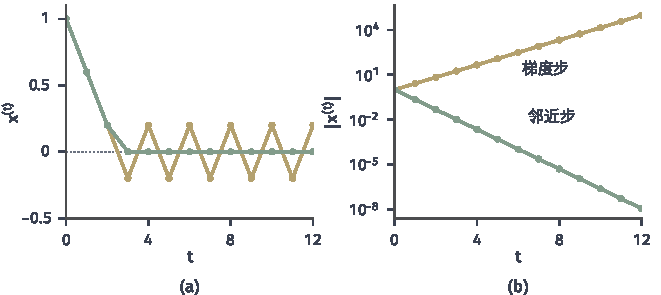
\includegraphics[width=112mm]{figures/05-optimization/03-nonsmooth-optimization/matplotlib/ns-forward-backward/figure.pdf}
  \caption{显式步（黄）与隐式的邻近步（绿）。$\alpha=0.4$，$x^{(0)}=1$。(a)$f(x)=\lvert x\rvert$：次梯度步在零点两侧反复跳动，邻近步第三步后停在零。(b)$f(x)=\tfrac92x^2$：$\alpha$超过$2/L=2/9$，梯度步发散，邻近步对任何$\alpha>0$都收缩，纵轴为对数坐标。}
  \label{fig:ns-forward-backward}
\end{BookInlineFigure}

第二个例子是二次函数$f(x)=\tfrac{c}{2}x^2$，$c=9$。显式与隐式的结果分别是
\[
 x^{+}=(1-\alpha c)x,\qquad x^{+}=\frac{x}{1+\alpha c}.
\]

$\alpha=0.4$时前者的放大倍数$\lvert1-3.6\rvert=2.6$，发散；后者的倍数$1/4.6$，收缩。隐式步对任意$\alpha>0$都不会过冲，见图~\ref{fig:ns-forward-backward}(b)。代价已经写在公式里：$\alpha c$大时要解一个方程，只不过一元时解起来很便宜。表~\ref{tab:ns-explicit-implicit}对比了两者。

\begin{BookInlineTable}
  \centering
  \small
  \begin{tabular}{@{}lll@{}}
    \toprule
     & 显式的梯度或次梯度步 & 隐式的邻近步\\
    \midrule
    更新 & $\bm{x}^{+}=\bm{x}-\alpha\bm{g}(\bm{x})$ & $\bm{x}^{+}=\bm{x}-\alpha\bm{s}$，$\bm{s}\in\partial f(\bm{x}^{+})$\\
    步长限制 & 光滑时$\alpha<2/L$ & 任意$\alpha>0$\\
    尖点 & 跨过去，来回振荡 & 可以停在尖点上\\
    每步代价 & 一次梯度或次梯度 & 解一个带二次项的子问题\\
    是否下降 & 非光滑时不一定 & 总是下降（或已最优）\\
    \bottomrule
  \end{tabular}
  \caption{显式步与隐式的邻近步。两者的数学形式相同，差别在于斜率取在哪个点上。}
  \label{tab:ns-explicit-implicit}
\end{BookInlineTable}

\paragraph{第一个例子：投影}
设$\bm{C}$是非空闭凸集，$f=\iota_{\bm{C}}$。约束指标函数在$\bm{C}$内为零，外面为$+\infty$，邻近子问题变成在$\bm{C}$里找离$\bm{x}$最近的点：
\begin{equation}
 \operatorname{prox}_{\alpha\iota_{\bm{C}}}(\bm{x})=\Pi_{\bm{C}}(\bm{x})=\argmin_{\bm{y}\in\bm{C}}\lVert\bm{y}-\bm{x}\rVert_2.
 \label{eq:ns-projection}
\end{equation}

结果与$\alpha$无关，因为函数值在$\bm{C}$内恒为零。这里$\iota_{\bm{C}}$适当、下半连续、凸的条件，正好要求$\bm{C}$非空、闭、凸。

由式~\eqref{eq:ns-prox-characterization}和式~\eqref{eq:ns-normal-cone}，$\bm{p}=\Pi_{\bm{C}}(\bm{x})$的特征是
\[
 \langle\bm{x}-\bm{p},\bm{y}-\bm{p}\rangle\leq0\qquad\text{对所有}\ \bm{y}\in\bm{C}.
\]
也就是从$\bm{p}$看，$\bm{x}$与$\bm{C}$中任一点的夹角不小于直角。

投影是否好算取决于$\bm{C}$。盒子逐坐标截断，球沿半径缩回。例如$\bm{C}=[-1,1]^2$时，$(2,0.5)$投影到$(1,0.5)$；单位球时，$(3,4)$投影到$(0.6,0.8)$。图~\ref{fig:ns-projection}画出了这两种情形。

\begin{BookInlineFigure}
  \centering
  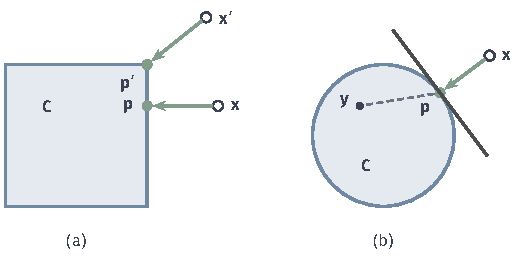
\includegraphics[width=88.4mm]{figures/05-optimization/03-nonsmooth-optimization/tikz/ns-projection/figure.pdf}
  \caption{投影是约束指标函数的邻近映射。浅蓝区域是$\bm{C}$，空心圆是输入点，绿点是投影。(a)盒约束逐坐标截断，$\bm{x}'$落在角上。(b)球约束，深灰线是过$\bm{p}$的切线。集合内任一点$\bm{y}$都在切线的同一侧，从$\bm{p}$看$\bm{x}$与$\bm{y}$夹角不小于直角。}
  \label{fig:ns-projection}
\end{BookInlineFigure}

\paragraph{第二个例子：软阈值}
取$f(y)=\lvert y\rvert$。由式~\eqref{eq:ns-prox-characterization}和式~\eqref{eq:ns-abs-subdiff}，按$p$的符号分三种情形。

若$p>0$，则$(x-p)/\alpha=1$，即$p=x-\alpha$，这要求$x>\alpha$。

若$p<0$，则$(x-p)/\alpha=-1$，即$p=x+\alpha$，这要求$x<-\alpha$。

若$p=0$，则$x/\alpha\in[-1,1]$，即$\lvert x\rvert\leq\alpha$。

三种情形恰好互斥且覆盖全部$x$，合起来得到\term{软阈值}（soft thresholding）算子：
\begin{equation}
 S_\alpha(x)=\operatorname{prox}_{\alpha\lvert\cdot\rvert}(x)=\operatorname{sign}(x)\max\{\lvert x\rvert-\alpha,\,0\}.
 \label{eq:ns-soft-threshold}
\end{equation}

它把靠近零的输入压成零，把其余的朝零移动$\alpha$。向量的$\ell_1$范数按坐标可分，邻近映射就是逐坐标软阈值。阈值由步长乘系数给出，$\alpha\lambda\lVert\cdot\rVert_1$的邻近映射就是逐坐标作用的$S_{\alpha\lambda}$。图~\ref{fig:ns-prox-geometry}的两个输入，由公式得$S_1(2)=1$，$S_1(0.6)=0$，都与图中相符。

图~\ref{fig:ns-prox-maps}(a)是这个映射的图像，粗线的长度$2\alpha$就是原点次微分的长度$2$乘$\alpha$。这条规律具有一般性。(b)是三段折线在$\alpha=1$的邻近映射，用同样的分情形方法，每个分支上$p=x-\alpha a_i$（$a_i$是斜率），两个尖点各对应一段水平线，长度分别是$\alpha$乘$\tfrac32$（$x\in[-1,\tfrac12]$）和$\alpha$乘$\tfrac32$（$x\in[\tfrac52,4]$），正好是$\partial f(0)$和$\partial f(2)$的长度乘$\alpha$。

\begin{BookInlineFigure}
  \centering
  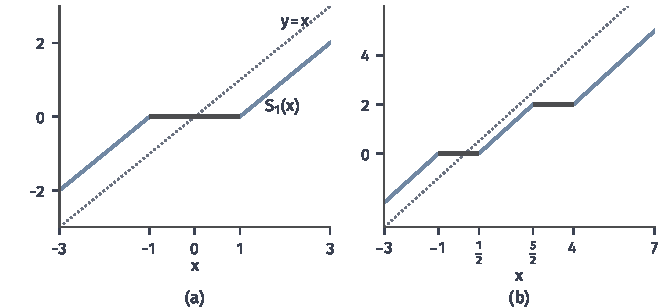
\includegraphics[width=112mm]{figures/05-optimization/03-nonsmooth-optimization/matplotlib/ns-prox-maps/figure.pdf}
  \caption{两个邻近映射的图像（$\alpha=1$），点线是恒等映射。(a)软阈值$S_1$，深灰粗线是被压成零的区间$[-1,1]$。(b)三段折线的邻近映射，深灰粗线是落在尖点$x=0$和$x=2$上的输入区间，长度等于对应次微分的长度乘$\alpha$。}
  \label{fig:ns-prox-maps}
\end{BookInlineFigure}

\subsection{邻近点法}
\label{sec:ns-proximal-point}

既然邻近映射把点往$f$低的方向移，反复应用它会怎样？\term{邻近点法}（proximal point method）就是
\begin{equation}
 \bm{x}^{(t+1)}=\operatorname{prox}_{\alpha^{(t)}f}(\bm{x}^{(t)}),\qquad\alpha^{(t)}>0.
 \label{eq:ns-ppa}
\end{equation}

这是把式~\eqref{eq:ns-implicit-step}反复迭代，每一步的位移除以步长都是新点的一个次梯度。下面的定理说明步长可以任意大，这是显式方法做不到的。

\begin{theorem}[邻近点法的目标差界]
\label{thm:ns-ppa}
设$f$是适当、下半连续的凸函数，存在最小点$\bm{x}^\star$，每一步精确计算式~\eqref{eq:ns-ppa}。则$f(\bm{x}^{(t)})$单调不增，并且
\begin{equation}
 f(\bm{x}^{(T)})-f^\star\leq\frac{\lVert\bm{x}^{(0)}-\bm{x}^\star\rVert_2^2}{2\sum_{t=0}^{T-1}\alpha^{(t)}}.
 \label{eq:ns-ppa-rate}
\end{equation}
\end{theorem}

\begin{proof}
省略上标，把第$t$步的点、新点和步长写成$\bm{x},\bm{x}^{+},\alpha$。由式~\eqref{eq:ns-prox-characterization}，向量$(\bm{x}-\bm{x}^{+})/\alpha$（记为$\bm{s}$）是$f$在$\bm{x}^{+}$的次梯度，所以对任意$\bm{z}$，
\[
 f(\bm{x}^{+})-f(\bm{z})\leq\langle\bm{s},\bm{x}^{+}-\bm{z}\rangle=\frac1\alpha\langle\bm{x}-\bm{x}^{+},\bm{x}^{+}-\bm{z}\rangle.
\]

取$\bm{z}=\bm{x}$，右端是$-\lVert\bm{x}^{+}-\bm{x}\rVert_2^2/\alpha\leq0$，单调性得证。

取$\bm{z}=\bm{x}^\star$，并使用恒等式
\begin{equation}
 2\langle\bm{a}-\bm{b},\bm{b}-\bm{c}\rangle=\lVert\bm{a}-\bm{c}\rVert_2^2-\lVert\bm{b}-\bm{c}\rVert_2^2-\lVert\bm{a}-\bm{b}\rVert_2^2,
 \label{eq:ns-three-point}
\end{equation}
得到
\[
 \alpha\bigl(f(\bm{x}^{+})-f^\star\bigr)\leq\frac12\Bigl(\lVert\bm{x}-\bm{x}^\star\rVert_2^2-\lVert\bm{x}^{+}-\bm{x}^\star\rVert_2^2\Bigr).
\]

对$t=0,\ldots,T-1$相加，距离项相消，右端不超过$\lVert\bm{x}^{(0)}-\bm{x}^\star\rVert_2^2/2$。左端由单调性，每一项的$f(\bm{x}^{(t+1)})\geq f(\bm{x}^{(T)})$，于是
\[
 \Bigl(\sum_{t=0}^{T-1}\alpha^{(t)}\Bigr)\bigl(f(\bm{x}^{(T)})-f^\star\bigr)\leq\frac12\lVert\bm{x}^{(0)}-\bm{x}^\star\rVert_2^2.
\]
两边相除即得。
\end{proof}

分母里是$\alpha^{(t)}$的累积，所以$\alpha$越大收敛越快。一步用很大的$\alpha$，子问题几乎就是原问题，这正是问题所在：式~\eqref{eq:ns-ppa}把难度搬进了子问题，并没有消除它。

用第~\ref{chap:first-order-methods}章的二次目标$f(\bm{x})=\tfrac12(x_1^2+9x_2^2)$，$\bm{x}^{(0)}=(9,1)$演示。对角情形的子问题有闭式解，$\alpha=1$时第一步是
\[
 \bm{x}^{(1)}=\Bigl(\frac{9}{1+1},\ \frac{1}{1+9}\Bigr)=(4.5,\,0.1).
\]

再走一步，
\[
 \bm{x}^{(2)}=(2.25,\,0.01).
\]

图~\ref{fig:ns-ppa-path}(a)中绿色路径没有梯度下降（黄色，$\alpha=1/5$）的折返，(b)说明$\alpha$增大时收敛更快。这个例子每步的工作量几乎为零，但只是因为$\bm{H}$是对角矩阵。一般二次目标的子问题是线性方程组$(\bm{I}+\alpha\bm{H})\bm{x}^{+}=\bm{x}$，$\alpha$越大，它的条件数越接近$\bm{H}$本身，求解代价越接近原问题。

\begin{BookInlineFigure}
  \centering
  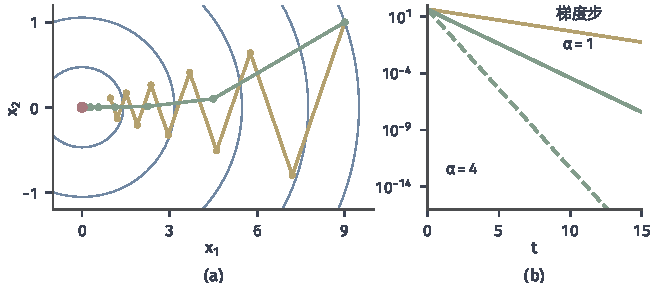
\includegraphics[width=112mm]{figures/05-optimization/03-nonsmooth-optimization/matplotlib/ns-ppa-path/figure.pdf}
  \caption{邻近点法在二次目标$\tfrac12(x_1^2+9x_2^2)$上的表现，$\bm{x}^{(0)}=(9,1)$。(a)等高线（蓝）上的路径，横纵比例不同，绿色为$\alpha=1$的邻近点法，黄色为$\alpha=1/5$的梯度下降。(b)目标差（对数坐标），绿色实线、虚线分别是$\alpha=1,4$的邻近点法，黄色是梯度下降。}
  \label{fig:ns-ppa-path}
\end{BookInlineFigure}

\paragraph{三件事要分别核验}
使用邻近点法时要分清三个问题，它们不能相互代替。

第一，映射可定义。这由定理~\ref{thm:ns-prox}回答，只要$f$适当、下半连续、凸。

第二，子问题可计算。定义合法不等于算得出来。对$\lvert x\rvert$有闭式解，对$\tfrac12(x_1^2+9x_2^2)$有简单公式；对一般的$f$，子问题本身需要迭代求解。

第三，原问题收敛。定理~\ref{thm:ns-ppa}额外要求最小点存在。取$f(x)=e^x$，邻近映射处处有定义，每一步也能用牛顿法算出。$\alpha=1$，$x^{(0)}=0$时，方程$p-x+e^p=0$依次给出
\[
 x^{(1)}\approx-0.567,\qquad x^{(2)}\approx-0.953,\qquad x^{(3)}\approx-1.242.
\]
序列单调趋于$-\infty$，$f(x^{(t)})$趋于下确界$0$，但下确界取不到，也就不存在“收敛到解”这回事。

\paragraph{子问题的精度}
实际中子问题只能算到一定精度。设计算结果与精确的邻近点的距离不超过$\varepsilon^{(t)}$。由非扩张性~\eqref{eq:ns-firm-nonexpansive}，$\bm{x}^\star$是不动点，所以
\begin{equation}
 \lVert\bm{x}^{(t+1)}-\bm{x}^\star\rVert_2\leq\lVert\bm{x}^{(t)}-\bm{x}^\star\rVert_2+\varepsilon^{(t)}.
 \label{eq:ns-inexact-prox}
\end{equation}

只要$\sum_t\varepsilon^{(t)}<\infty$，这个递推就说明序列有界，误差的累积不会把点推走。进一步可证，在$\alpha^{(t)}$有正下界时序列收敛到一个最小点，证明要用到不动点序列的单调性论证，篇幅较长。

若误差不衰减，结果只能到某个精度。用$f(x)=\lvert x\rvert$，$\alpha=0.4$，$x^{(0)}=1$，假设每一步都多偏出$0.1$：
\[
 1\ \to\ 0.7\ \to\ 0.4\ \to\ 0.1\ \to\ 0.1\ \to\cdots
\]
序列停在$0.1$。这里的$0.1$恰好是子问题的误差。把误差取成$\varepsilon^{(t)}=0.1\cdot2^{-t}$后，点最终收敛到零。子问题要算多准，取决于最后想要多准，二者是同一量级的问题，这个经验在后面的邻近梯度法上同样适用。

\section{复合优化}
\label{sec:ns-composite}

Lasso的目标一半是光滑的最小二乘，一半是带尖点的$\ell_1$范数。对整个目标用次梯度法，浪费了光滑项的信息；对整个目标用邻近点法，子问题和原问题一样难。能否只线性化光滑的一半，把有尖点的一半原样留下，并得到比次梯度法快得多的保证？

考虑\term{复合目标}（composite objective）
\begin{equation}
 F(\bm{x})=f(\bm{x})+r(\bm{x}),
 \label{eq:ns-composite}
\end{equation}
其中$f:\mathbb{R}^n\to\mathbb{R}$可微且梯度$L$-Lipschitz连续，$r$是适当、下半连续的凸函数，并且$\operatorname{prox}_{\alpha r}$容易计算。计算上的约定是：读$\nabla f$和计算$\operatorname{prox}_{\alpha r}$都可以负担，但对$f+r$整体的邻近映射算不了。

\subsection{邻近梯度法}
\label{sec:ns-proximal-gradient}

\paragraph{主要思想}
由第~\ref{chap:smooth-foundations}章的下降引理，当$0<\alpha\leq1/L$时，光滑项有二次上界
\[
 f(\bm{y})\leq f(\bm{x})+\langle\nabla f(\bm{x}),\bm{y}-\bm{x}\rangle+\frac{1}{2\alpha}\lVert\bm{y}-\bm{x}\rVert_2^2.
\]

把$F$中的$f$换成这个上界，$r$一字不动，得到当前点$\bm{x}^{(t)}$处的模型：
\begin{equation}
 m^{(t)}(\bm{y})=f(\bm{x}^{(t)})+\langle\nabla f(\bm{x}^{(t)}),\bm{y}-\bm{x}^{(t)}\rangle+\frac{1}{2\alpha}\lVert\bm{y}-\bm{x}^{(t)}\rVert_2^2+r(\bm{y}).
 \label{eq:ns-composite-model}
\end{equation}

模型中与$\bm{y}$有关的一次项和二次项可以配方：
\[
 \langle\nabla f(\bm{x}),\bm{y}-\bm{x}\rangle+\frac{1}{2\alpha}\lVert\bm{y}-\bm{x}\rVert_2^2
 =\frac{1}{2\alpha}\bigl\lVert\bm{y}-\bigl(\bm{x}-\alpha\nabla f(\bm{x})\bigr)\bigr\rVert_2^2-\frac{\alpha}{2}\lVert\nabla f(\bm{x})\rVert_2^2.
\]

去掉不含$\bm{y}$的项，模型的最小点就是从梯度步的终点出发求$r$的邻近映射。这就是\term{邻近梯度法}（proximal gradient method）：
\begin{equation}
 \bm{x}^{(t+1)}=\operatorname{prox}_{\alpha r}\bigl(\bm{x}^{(t)}-\alpha\nabla f(\bm{x}^{(t)})\bigr).
 \label{eq:ns-prox-grad}
\end{equation}

它分两步看：光滑项做显式的梯度步，非光滑项做隐式的邻近步。图~\ref{fig:ns-composite-model}用一维的$F(x)=\tfrac12(x-2)^2+\tfrac12\lvert x\rvert$（$L=1$）展示模型的作用。绿色虚线在原点处有与$F$相同的尖点，这是把$r$留在模型里的直接效果。(a)的$\alpha=0.5\leq1/L$，模型处处高于$F$，最小化模型一定使$F$下降，这与第~\ref{chap:smooth-foundations}章的下降引理是同一个道理。(b)的$\alpha=2.5>1/L$，模型不再是上界，它的最小点跑到了$F$更高的地方。

\begin{BookInlineFigure}
  \centering
  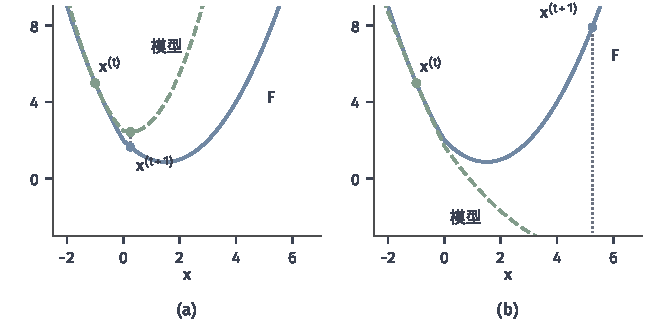
\includegraphics[width=112mm]{figures/05-optimization/03-nonsmooth-optimization/matplotlib/ns-composite-model/figure.pdf}
  \caption{复合目标的局部模型，$F(x)=\tfrac12(x-2)^2+\tfrac12\lvert x\rvert$，$L=1$，当前点$x^{(t)}=-1$。蓝线是$F$，绿色虚线是式~\eqref{eq:ns-composite-model}的模型，蓝点是新点处的真实目标值。(a)$\alpha=0.5$，模型在$F$上方，新点$x^{(t+1)}=0.25$处$F$从$5$降到约$1.66$。(b)$\alpha=2.5$，模型部分低于$F$，新点$x^{(t+1)}=5.25$处$F$升到约$7.9$。}
  \label{fig:ns-composite-model}
\end{BookInlineFigure}

式~\eqref{eq:ns-prox-grad}包含几种已知情形：$r=0$时是梯度下降；$f=0$时是邻近点法；$r=\iota_{\bm{C}}$时是投影梯度法，集合的计算和可行点的最优性将在第~\ref{chap:feasible-iterations}章讨论。

取$r=\lambda\lVert\cdot\rVert_1$（$\lambda>0$），$f$为Lasso的最小二乘项，$\nabla f(\bm{x})=\bm{A}^\top(\bm{A}\bm{x}-\bm{b})$，$L=\lVert\bm{A}\rVert_2^2$。由软阈值式~\eqref{eq:ns-soft-threshold}，邻近步的阈值是步长乘$\lambda$，式~\eqref{eq:ns-prox-grad}成为
\begin{equation}
 \bm{x}^{(t+1)}=S_{\alpha\lambda}\bigl(\bm{x}^{(t)}-\alpha\bm{A}^\top(\bm{A}\bm{x}^{(t)}-\bm{b})\bigr).
 \label{eq:ns-ista}
\end{equation}

这种迭代称为\term{迭代软阈值算法}（iterative shrinkage-thresholding algorithm，ISTA）。“迭代”和“阈值”正好是它的两步：先按最小二乘的方向修正系数，再把小的系数压成零。

\paragraph{计算过程}
用章首的例~\eqref{eq:ns-lasso-example}。

\needspace{6\baselineskip}
\paragraph{变量}
\begin{itemize}
 \item $\bm{A}\in\mathbb{R}^{p\times n}$，$\bm{b}\in\mathbb{R}^p$，$\lambda>0$：数据。例中$p=3$，$n=2$，$\lambda=1$。
 \item $\bm{x}^{(t)}\in\mathbb{R}^n$：当前点。
 \item $\bm{g}^{(t)}$：光滑项在当前点的梯度。
 \item $\alpha$：步长，$\alpha\leq1/L$。
\end{itemize}

\paragraph{初始化}
选$\bm{x}^{(0)}$和$\alpha$。例中$\bm{A}^\top\bm{A}$和$\bm{A}^\top\bm{b}$分别是
\[
 \bm{A}^\top\bm{A}=\begin{pmatrix}2&1\\1&2\end{pmatrix},\qquad\bm{A}^\top\bm{b}=\begin{pmatrix}5\\2\end{pmatrix}.
\]
$\bm{A}^\top\bm{A}$的特征值是$3$和$1$，所以$L=3$。取$\alpha=1/3$，$\bm{x}^{(0)}=(0,0)$，阈值$\alpha\lambda=1/3$。

\needspace{6\baselineskip}
\paragraph{每轮更新}
\begin{enumerate}
 \item 算梯度，$\bm{g}^{(t)}$等于$\bm{A}^\top\bm{A}\bm{x}^{(t)}$减去$\bm{A}^\top\bm{b}$。例中第一轮
 \[
  \bm{g}^{(0)}=(-5,-2).
 \]
 \item 走梯度步$\bm{z}^{(t)}=\bm{x}^{(t)}-\alpha\bm{g}^{(t)}$。例中第一轮
 \[
  \bm{z}^{(0)}=\Bigl(\frac53,\ \frac23\Bigr).
 \]
 \item 逐坐标软阈值，由式~\eqref{eq:ns-ista}得新点。例中第一轮
 \[
  \bm{x}^{(1)}=\Bigl(\frac43,\ \frac13\Bigr),\qquad F(\bm{x}^{(1)})=\frac{11}{3}.
 \]
\end{enumerate}

第二轮的三个量依次是
\[
 \bm{g}^{(1)}=(-2,\,0),\qquad\bm{z}^{(1)}=\Bigl(2,\ \frac13\Bigr),\qquad\bm{x}^{(2)}=\Bigl(\frac53,\ 0\Bigr).
\]

第二分量恰好被压到零。第三轮的三个量依次是
\[
 \bm{g}^{(2)}=\Bigl(-\frac53,\,-\frac13\Bigr),\qquad\bm{z}^{(2)}=\Bigl(\frac{20}{9},\ \frac19\Bigr),\qquad\bm{x}^{(3)}=\Bigl(\frac{17}{9},\ 0\Bigr).
\]

此后第二分量一直为零：$\bm{z}$的第二分量是$(2-x_1)/3$，绝对值小于阈值$1/3$。第一分量满足$x_1^{+}=x_1/3+4/3$，每轮把与$2$的距离缩小三分之一。目标差依次是
\[
 \frac23,\qquad\frac19,\qquad\frac{1}{81},\qquad\frac{1}{729},\ldots
\]

达到预定的迭代次数或后面第~\ref{sec:ns-stopping}小节的停止条件后结束，最终得到$\bm{x}^{(T)}\to(2,0)$，也就是第~\ref{sec:ns-subdifferential}节验证的解。

\paragraph{收敛分析}
分析的核心是一步不等式，把式~\eqref{eq:ns-prox-characterization}与下降引理结合。

\begin{lemma}[邻近梯度的一步不等式]
\label{lem:ns-pg-one-step}
设$f$凸且可微，$r$是适当、下半连续的凸函数，$F=f+r$。给定$\bm{y}$与$\alpha>0$，令
\begin{equation}
 \bm{x}^{+}=\operatorname{prox}_{\alpha r}\bigl(\bm{y}-\alpha\nabla f(\bm{y})\bigr).
 \label{eq:ns-pg-step-y}
\end{equation}
若
\begin{equation}
 f(\bm{x}^{+})\leq f(\bm{y})+\langle\nabla f(\bm{y}),\bm{x}^{+}-\bm{y}\rangle+\frac{1}{2\alpha}\lVert\bm{x}^{+}-\bm{y}\rVert_2^2,
 \label{eq:ns-backtrack-condition}
\end{equation}
则对任意$\bm{z}\in\operatorname{dom}F$，
\begin{equation}
 F(\bm{x}^{+})-F(\bm{z})\leq\frac{1}{2\alpha}\Bigl(\lVert\bm{y}-\bm{z}\rVert_2^2-\lVert\bm{x}^{+}-\bm{z}\rVert_2^2\Bigr).
 \label{eq:ns-pg-one-step}
\end{equation}
\end{lemma}

\begin{proof}
$f$的凸性给出下界
\[
 f(\bm{y})+\langle\nabla f(\bm{y}),\bm{z}-\bm{y}\rangle\leq f(\bm{z}).
\]
把它代入式~\eqref{eq:ns-backtrack-condition}，
\[
 f(\bm{x}^{+})\leq f(\bm{z})+\langle\nabla f(\bm{y}),\bm{x}^{+}-\bm{z}\rangle+\frac{1}{2\alpha}\lVert\bm{x}^{+}-\bm{y}\rVert_2^2.
\]

由式~\eqref{eq:ns-prox-characterization}和式~\eqref{eq:ns-pg-step-y}，下面的$\bm{s}$是$r$在$\bm{x}^{+}$的次梯度：
\[
 \bm{s}=\frac{\bm{y}-\bm{x}^{+}}{\alpha}-\nabla f(\bm{y}).
\]
所以
\[
 r(\bm{x}^{+})\leq r(\bm{z})+\langle\bm{s},\bm{x}^{+}-\bm{z}\rangle.
\]

两式相加，$\nabla f(\bm{y})$的项相消，得到
\[
 F(\bm{x}^{+})\leq F(\bm{z})+\frac{1}{\alpha}\langle\bm{y}-\bm{x}^{+},\bm{x}^{+}-\bm{z}\rangle+\frac{1}{2\alpha}\lVert\bm{x}^{+}-\bm{y}\rVert_2^2.
\]

再用恒等式~\eqref{eq:ns-three-point}，令$\bm{a}=\bm{y}$，$\bm{b}=\bm{x}^{+}$，$\bm{c}=\bm{z}$，最后一项被抵消，就是式~\eqref{eq:ns-pg-one-step}。
\end{proof}

条件~\eqref{eq:ns-backtrack-condition}只在$\bm{y}$和$\bm{x}^{+}$这一对点上要求上界成立，$\alpha\leq1/L$时自动满足。下面的结论就是这个引理对$\bm{y}=\bm{x}^{(t)}$的累加。

\begin{theorem}[邻近梯度法的收敛速率]
\label{thm:ns-pg-rate}
设$f$凸，梯度$L$-Lipschitz连续，$r$是适当、下半连续的凸函数，$F$存在最小点$\bm{x}^\star$，每步精确计算邻近映射，$0<\alpha\leq1/L$。则$F(\bm{x}^{(t)})$单调不增，并且
\begin{equation}
 F(\bm{x}^{(T)})-F^\star\leq\frac{\lVert\bm{x}^{(0)}-\bm{x}^\star\rVert_2^2}{2\alpha T}.
 \label{eq:ns-pg-rate}
\end{equation}
\end{theorem}

\begin{proof}
在式~\eqref{eq:ns-pg-one-step}中取$\bm{y}=\bm{z}=\bm{x}^{(t)}$（$t\geq1$时$\bm{x}^{(t)}\in\operatorname{dom}F$），右端为负，所以$F$单调不增。

取$\bm{y}=\bm{x}^{(t)}$，$\bm{z}=\bm{x}^\star$，对$t=0,\ldots,T-1$相加，距离项相消，得到
\[
 \sum_{t=0}^{T-1}\bigl(F(\bm{x}^{(t+1)})-F^\star\bigr)\leq\frac{\lVert\bm{x}^{(0)}-\bm{x}^\star\rVert_2^2}{2\alpha}.
\]

由单调性，左端每一项都不小于$F(\bm{x}^{(T)})-F^\star$，所以左端不小于$T(F(\bm{x}^{(T)})-F^\star)$，即得式~\eqref{eq:ns-pg-rate}。
\end{proof}

速率$O(1/T)$与第~\ref{chap:first-order-methods}章的梯度下降相同，比次梯度法的$O(1/\sqrt{T})$快得多，代价是$r$的邻近映射必须算得出。这里$\bm{x}^{(0)}$若不在$\operatorname{dom}r$，第一步的邻近映射会把点带入定义域，定理依然成立。

例中$R^2=\lVert\bm{x}^{(0)}-\bm{x}^\star\rVert_2^2=4$，$\alpha=1/3$，界为$6/T$，$T=3$时为$2$。实际目标差$1/81$小得多，因为一旦$x_2$落到零，迭代实际上在一维的强凸二次函数上运行，收敛是线性的。这也是Lasso上常见的现象：大多数轮次之后，支撑集（非零分量的位置）不再变化，算法此后近似一个定义在支撑集上的光滑问题。

\subsection{加速邻近梯度法（FISTA）}
\label{sec:ns-fista}

第~\ref{chap:first-order-methods}章的Nesterov方法把光滑凸目标的速率从$1/T$提高到$1/T^2$，代价只是多存一个向量。本小节要回答：这种外推能否直接搬到复合目标上？

\paragraph{主要思想}
把Nesterov方法里的梯度步换成邻近梯度步，外推系数原样保留。这就是\term{加速邻近梯度法}（fast iterative shrinkage-thresholding algorithm，FISTA）\scite{beck2009fista}：
\begin{equation}
 \begin{aligned}
 \bm{x}^{(t+1)}&=\operatorname{prox}_{\alpha r}\bigl(\bm{y}^{(t)}-\alpha\nabla f(\bm{y}^{(t)})\bigr),\\
 \bm{y}^{(t+1)}&=\bm{x}^{(t+1)}+\frac{\theta^{(t)}-1}{\theta^{(t+1)}}\bigl(\bm{x}^{(t+1)}-\bm{x}^{(t)}\bigr).
 \end{aligned}
 \label{eq:ns-fista}
\end{equation}

其中$\bm{y}^{(0)}=\bm{x}^{(0)}$，$\theta^{(0)}=1$，外推参数按第~\ref{chap:first-order-methods}章的递推更新：
\begin{equation}
 \theta^{(t+1)}=\frac{1+\sqrt{1+4(\theta^{(t)})^2}}{2}.
 \label{eq:ns-fista-theta}
\end{equation}
图~\ref{fig:ns-fista-structure}是一步的结构：先沿上一步位移外推到$\bm{y}^{(t)}$，在外推点读梯度，再做邻近步。梯度必须取在$\bm{y}^{(t)}$，这是Nesterov方法的特点，与重球法不同。

\begin{BookInlineFigure}
  \centering
  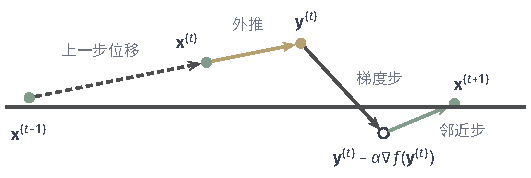
\includegraphics[width=89.9mm]{figures/05-optimization/03-nonsmooth-optimization/tikz/ns-fista-structure/figure.pdf}
  \caption{FISTA的一步。黄色外推从$\bm{x}^{(t)}$沿上一步位移（虚线）走到$\bm{y}^{(t)}$，深灰箭头是在$\bm{y}^{(t)}$处的梯度步，绿色箭头是邻近步，可能把点压回坐标面（深灰横线）。空心圆是梯度步的终点。}
  \label{fig:ns-fista-structure}
\end{BookInlineFigure}

\paragraph{计算过程}
仍用例~\eqref{eq:ns-lasso-example}，$\alpha=1/3$，阈值$1/3$。

\needspace{6\baselineskip}
\paragraph{变量}
\begin{itemize}
 \item $\bm{x}^{(t)}$：邻近步的输出，是算法报告的点。
 \item $\bm{y}^{(t)}$：外推点，形状与$\bm{x}$相同，读梯度在这里。
 \item $\theta^{(t)}$：外推参数。
\end{itemize}

\paragraph{初始化}
$\bm{x}^{(0)}=\bm{y}^{(0)}=\bm{0}$，$\theta^{(0)}=1$。

\needspace{6\baselineskip}
\paragraph{每轮更新}
\begin{enumerate}
 \item 在$\bm{y}^{(t)}$读梯度并做邻近梯度步，由式~\eqref{eq:ns-fista}得$\bm{x}^{(t+1)}$。例中第一轮$\bm{y}^{(0)}=\bm{0}$，结果与ISTA相同：
 \[
  \bm{x}^{(1)}=\Bigl(\frac43,\ \frac13\Bigr).
 \]
 \item 更新$\theta^{(t+1)}$。例中第一轮
 \[
  \theta^{(1)}=\frac{1+\sqrt5}{2}\approx1.618.
 \]
 \item 计算外推点。例中第一轮系数$(\theta^{(0)}-1)/\theta^{(1)}=0$，所以$\bm{y}^{(1)}=\bm{x}^{(1)}$。
\end{enumerate}

第二轮仍无外推差别，同样得到$\bm{x}^{(2)}=(5/3,0)$。这时开始用上外推，
\[
 \theta^{(2)}\approx2.194,\qquad\frac{\theta^{(1)}-1}{\theta^{(2)}}\approx0.282.
\]

外推点是
\[
 \bm{y}^{(2)}=\Bigl(\frac53,0\Bigr)+0.282\Bigl(\frac13,-\frac13\Bigr)\approx(1.761,\,-0.094).
\]

第三轮的梯度、梯度步和新点依次是
\[
 \begin{gathered}
 \nabla f(\bm{y}^{(2)})\approx(-1.573,\,-0.427),\qquad
 \bm{z}\approx(2.285,\,0.048),\\
 \bm{x}^{(3)}\approx(1.952,\,0).
 \end{gathered}
\]

与ISTA的$17/9\approx1.889$相比更接近$2$，目标差约$0.0024$，ISTA是$0.0123$。外推的好处在第三轮就看得到了。

继续迭代，第一分量在第$4$轮越过$2$到达约$2.025$，然后缓慢摆回，目标差从第$7$轮的约$1.2\times10^{-6}$升到第$8$轮的约$4.4\times10^{-6}$。这个小问题上$\kappa=3$，ISTA已经很快，FISTA并不占优，但它显示了FISTA的目标值不是逐轮下降的。图~\ref{fig:ns-ista-path}对比了两条路径。

\begin{BookInlineFigure}
  \centering
  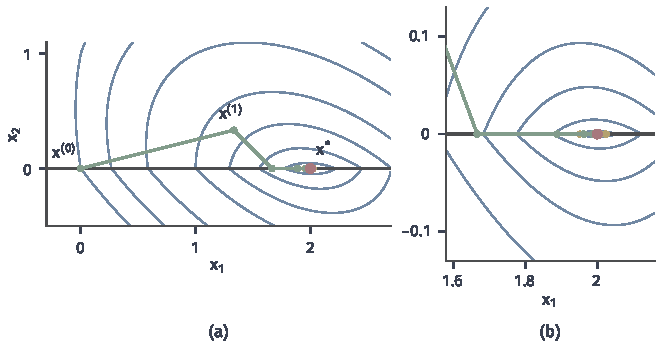
\includegraphics[width=112mm]{figures/05-optimization/03-nonsmooth-optimization/matplotlib/ns-ista-path/figure.pdf}
  \caption{贯穿例~\eqref{eq:ns-lasso-example}上的ISTA（绿）与FISTA（黄），蓝线是$F$的等高线，深灰横线是尖点所在的$x_2=0$。(a)全貌，迭代很快落到$x_2=0$上，等高线在这条线上带角。(b)$\bm{x}^\star=(2,0)$附近放大，FISTA越过红点后又摆回。}
  \label{fig:ns-ista-path}
\end{BookInlineFigure}

\paragraph{收敛分析}
结论的形式与第~\ref{chap:first-order-methods}章相同，证明把那里的一步不等式换成引理~\ref{lem:ns-pg-one-step}。我们把比较点写成任意的$\bm{z}$，后面分析光滑化时要用这个写法。

\begin{theorem}[FISTA的收敛速率]
\label{thm:ns-fista-rate}
设$f$凸，梯度$L$-Lipschitz连续，$r$是适当、下半连续的凸函数，每步精确计算邻近映射，$\alpha=1/L$，$\theta^{(t)}$按式~\eqref{eq:ns-fista-theta}递推。则对任意$\bm{z}\in\operatorname{dom}F$和$T\geq1$，
\begin{equation}
 F(\bm{x}^{(T)})-F(\bm{z})\leq\frac{2L\lVert\bm{x}^{(0)}-\bm{z}\rVert_2^2}{(T+1)^2}.
 \label{eq:ns-fista-rate}
\end{equation}
特别地，若$F$存在最小点$\bm{x}^\star$，取$\bm{z}=\bm{x}^\star$就得到目标差界。
\end{theorem}

\begin{proof}
记$\theta=\theta^{(t)}$，$\Delta_t$为目标差$F(\bm{x}^{(t)})-F(\bm{z})$。在引理~\ref{lem:ns-pg-one-step}中取$\bm{y}=\bm{y}^{(t)}$，$\bm{x}^{+}=\bm{x}^{(t+1)}$，比较点取
\[
 \bm{v}=\Bigl(1-\frac1\theta\Bigr)\bm{x}^{(t)}+\frac1\theta\bm{z}.
\]

由$F$的凸性，
\[
 F(\bm{v})-F(\bm{z})\leq\Bigl(1-\frac1\theta\Bigr)\Delta_t.
\]

代入式~\eqref{eq:ns-pg-one-step}，并记$\alpha=1/L$，得
\[
 \Delta_{t+1}-\Bigl(1-\frac1\theta\Bigr)\Delta_t\leq\frac L2\Bigl(\lVert\bm{y}^{(t)}-\bm{v}\rVert_2^2-\lVert\bm{x}^{(t+1)}-\bm{v}\rVert_2^2\Bigr).
\]

两边乘$\theta^2$，把$\theta$乘进范数。定义
\[
 \bm{u}^{(t+1)}=\theta^{(t)}\bm{x}^{(t+1)}-(\theta^{(t)}-1)\bm{x}^{(t)}-\bm{z},
\]
则$\theta\bm{x}^{(t+1)}-\theta\bm{v}=\bm{u}^{(t+1)}$。

再看另一项。令$\bm{u}^{(0)}=\bm{x}^{(0)}-\bm{z}$。由外推式~\eqref{eq:ns-fista}，$t\geq1$时有
\[
 \theta^{(t)}\bm{y}^{(t)}=\theta^{(t)}\bm{x}^{(t)}+(\theta^{(t-1)}-1)(\bm{x}^{(t)}-\bm{x}^{(t-1)}),
\]
于是
\[
 \theta\bm{y}^{(t)}-\theta\bm{v}=\bm{u}^{(t)}.
\]
$t=0$时$\theta^{(0)}=1$，$\bm{y}^{(0)}=\bm{x}^{(0)}$，同一等式也成立。

由递推，$\theta^2-\theta=(\theta^{(t-1)})^2$（$t\geq1$），而$t=0$时$\theta^2-\theta=0$。代入不等式，得到势函数的单调性：
\[
 (\theta^{(t)})^2\Delta_{t+1}+\frac L2\lVert\bm{u}^{(t+1)}\rVert_2^2\leq(\theta^{(t-1)})^2\Delta_t+\frac L2\lVert\bm{u}^{(t)}\rVert_2^2.
\]

把它从$t=T-1$一直用到$t=0$，最后一步$\theta^2-\theta=0$使$\Delta_0$的项消失，于是
\[
 (\theta^{(T-1)})^2\Delta_T\leq\frac L2\lVert\bm{x}^{(0)}-\bm{z}\rVert_2^2.
\]

由$\theta^{(t)}\geq(t+2)/2$得$(\theta^{(T-1)})^2\geq(T+1)^2/4$，代入即得结论。
\end{proof}

证明里没有用到$\Delta_t$的符号，这也是比较点可以取任意$\bm{z}$的原因。下面三点是使用时要注意的。第一，界里的$F(\bm{x}^{(T)})$不要求逐轮下降，例中第$8$轮的回升就是证据；若需要单调，可以在每轮比较后保留较好的点，但这样改过的算法需要另外分析。第二，$\alpha=1/L$可以换成回溯，但证明要求步长不增。第三，这个证明用到$F$的凸性（比较点$\bm{v}$的那一步），不能直接用于非凸的$f$。

图~\ref{fig:ns-ista-fista-rates}用一个条件更差的问题（$100\times200$的相关设计矩阵）比较两种方法。ISTA在这种问题上明显受制于条件数，FISTA在更少的迭代内到达更低的目标差，代价是目标值的振荡。

\begin{BookInlineFigure}
  \centering
  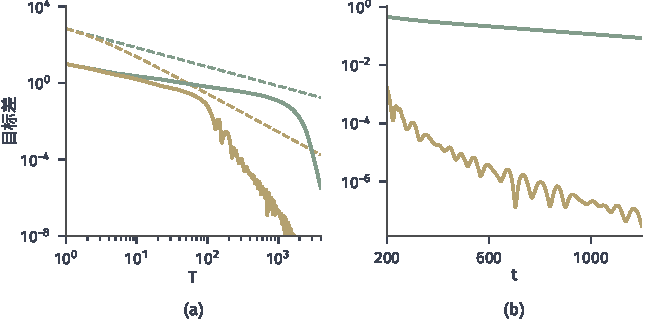
\includegraphics[width=112mm]{figures/05-optimization/03-nonsmooth-optimization/matplotlib/ns-ista-fista-rates/figure.pdf}
  \caption{相关设计的Lasso上的ISTA（绿）与FISTA（黄）。$\bm{A}\in\mathbb{R}^{100\times200}$的列间相关系数$\rho=0.9$，$\lambda$取为$0.005\lVert\bm{A}^\top\bm{b}\rVert_\infty$，$\alpha=1/L$。(a)目标差（双对数），同色虚线是定理~\ref{thm:ns-pg-rate}与定理~\ref{thm:ns-fista-rate}的上界。(b)第$200$到第$1200$轮的放大（半对数），FISTA的目标差呈周期性振荡，ISTA单调下降。最优值由高精度运行得到。}
  \label{fig:ns-ista-fista-rates}
\end{BookInlineFigure}

\subsection{停止条件与计算成本}
\label{sec:ns-stopping}

算法要在不知道$F^\star$的情况下决定何时停止。无约束光滑问题有$\lVert\nabla f\rVert_2$，复合目标在尖点上没有梯度，需要一个可计算的残差。本小节回答：这个残差是什么，它小意味着什么，以及比较算法时要算哪些账。

\paragraph{邻近梯度映射}
把一步更新的位移除以步长，定义\term{邻近梯度映射}（proximal gradient mapping）
\begin{equation}
 \bm{G}_\alpha(\bm{x})=\frac{1}{\alpha}\Bigl(\bm{x}-\operatorname{prox}_{\alpha r}\bigl(\bm{x}-\alpha\nabla f(\bm{x})\bigr)\Bigr).
 \label{eq:ns-gradient-mapping}
\end{equation}

$r=0$时它就是$\nabla f(\bm{x})$，所以它是梯度在复合目标上的替身。更新可以写成$\bm{x}^{+}=\bm{x}-\alpha\bm{G}_\alpha(\bm{x})$，这样它和梯度步在形式上完全一样。第~\ref{chap:optimization}章提到的非光滑问题的最优性残差，就是这个量。

满足$\bm{0}\in\nabla f(\bm{x})+\partial r(\bm{x})$的点称为\term{复合驻点}（composite stationary point）。这个定义不要求$f$凸。

\begin{theorem}[映射残差的含义]
\label{thm:ns-residual}
设$f$梯度$L$-Lipschitz连续，$r$是适当、下半连续的凸函数，$\alpha>0$，$\bm{x}^{+}=\bm{x}-\alpha\bm{G}_\alpha(\bm{x})$。
\begin{enumerate}
 \item $\bm{G}_\alpha(\bm{x})=\bm{0}$当且仅当$\bm{x}$是复合驻点。
 \item 若$f$凸且$\bm{G}_\alpha(\bm{x})=\bm{0}$，则$\bm{x}$是$F$的全局最小点。
 \item 若$\alpha L\leq1$，则$\bm{G}_\alpha(\bm{x})+\nabla f(\bm{x}^{+})-\nabla f(\bm{x})\in\nabla f(\bm{x}^{+})+\partial r(\bm{x}^{+})$，且范数不超过$2\lVert\bm{G}_\alpha(\bm{x})\rVert_2$。$f$凸且最小点$\bm{x}^\star$存在时，
 \begin{equation}
  F(\bm{x}^{+})-F^\star\leq2\lVert\bm{G}_\alpha(\bm{x})\rVert_2\,\lVert\bm{x}^{+}-\bm{x}^\star\rVert_2.
  \label{eq:ns-residual-gap}
 \end{equation}
 \item 不要求$f$凸，$\alpha=1/L$，$F$有下界$F_{\inf}$时，邻近梯度法满足
 \begin{equation}
  \min_{0\leq t<T}\lVert\bm{G}_\alpha(\bm{x}^{(t)})\rVert_2^2\leq\frac{2L\bigl(F(\bm{x}^{(0)})-F_{\inf}\bigr)}{T}.
  \label{eq:ns-nonconvex-residual}
 \end{equation}
\end{enumerate}
\end{theorem}

\begin{proof}
由式~\eqref{eq:ns-prox-characterization}，$\bm{x}^{+}$由下式刻画：
\[
 \bm{G}_\alpha(\bm{x})-\nabla f(\bm{x})\in\partial r(\bm{x}^{+}).
\]

第一条：$\bm{G}_\alpha(\bm{x})=\bm{0}$时$\bm{x}^{+}=\bm{x}$，上式就是$-\nabla f(\bm{x})\in\partial r(\bm{x})$。反过来，若$-\nabla f(\bm{x})\in\partial r(\bm{x})$，则由式~\eqref{eq:ns-prox-characterization}，$\bm{x}$本身就是$\bm{x}-\alpha\nabla f(\bm{x})$的邻近点，所以$\bm{x}^{+}=\bm{x}$。

第二条：$f$凸时$\partial F=\nabla f+\partial r$，用定理~\ref{thm:ns-fermat}。

第三条：在上式两边加$\nabla f(\bm{x}^{+})$就得到前半部分。范数方面，
\[
 \lVert\nabla f(\bm{x}^{+})-\nabla f(\bm{x})\rVert_2\leq L\lVert\bm{x}^{+}-\bm{x}\rVert_2=L\alpha\lVert\bm{G}_\alpha(\bm{x})\rVert_2\leq\lVert\bm{G}_\alpha(\bm{x})\rVert_2.
\]
$f$凸时这个向量是$F$在$\bm{x}^{+}$的次梯度，用支撑不等式和Cauchy不等式，得到式~\eqref{eq:ns-residual-gap}。

第四条：由刻画式和次梯度不等式，
\[
 r(\bm{x})\geq r(\bm{x}^{+})+\langle\bm{G}_\alpha(\bm{x})-\nabla f(\bm{x}),\bm{x}-\bm{x}^{+}\rangle.
\]

代入$\bm{x}-\bm{x}^{+}=\alpha\bm{G}_\alpha(\bm{x})$。再用下降引理
\[
 f(\bm{x}^{+})\leq f(\bm{x})+\langle\nabla f(\bm{x}),\bm{x}^{+}-\bm{x}\rangle+\frac L2\lVert\bm{x}^{+}-\bm{x}\rVert_2^2.
\]
两式相加，当$\alpha=1/L$时得到
\[
 F(\bm{x}^{+})\leq F(\bm{x})-\frac{1}{2L}\lVert\bm{G}_\alpha(\bm{x})\rVert_2^2.
\]
对$t$求和，就是式~\eqref{eq:ns-nonconvex-residual}。
\end{proof}

第三条给出了可计算的证书：$\bm{x}^{+}$处的一个具体的次梯度，其范数不超过$2\lVert\bm{G}\rVert$。第四条说明非凸时没有目标差界，只能保证残差变小，这与光滑非凸问题的情况相同。

非凸时残差为零不代表最优。取$f(x)=-x^2/2$，$r=\iota_{[-1,1]}$，$L=1$，$\alpha=1$，则
\[
 G_1(x)=x-\Pi_{[-1,1]}(2x).
\]
$x=0$处$G_1=0$，但$0$是这个问题的最大点，真正的最优解在$\pm1$。

用贯穿例核对第三条。ISTA在$\bm{x}^{(3)}=(17/9,0)$处的下一步是$\bm{x}^{(4)}=(53/27,0)$，所以
\[
 \bm{G}_{1/3}(\bm{x}^{(3)})=3\Bigl(\frac{17}{9}-\frac{53}{27},\ 0\Bigr)=\Bigl(-\frac29,\ 0\Bigr).
\]

式~\eqref{eq:ns-residual-gap}的右端是$2\cdot\tfrac29\cdot\tfrac{1}{27}\approx0.0165$，实际$F(\bm{x}^{(4)})-F^\star\approx0.00137$，上界成立。

\paragraph{停止条件}
实际常用的停止条件是残差相对于初始残差足够小：
\begin{equation}
 \lVert\bm{G}_\alpha(\bm{x}^{(t)})\rVert_2\leq\varepsilon\max\bigl\{1,\lVert\bm{G}_\alpha(\bm{x}^{(0)})\rVert_2\bigr\}.
 \label{eq:ns-stopping}
\end{equation}

FISTA的邻近梯度步是在$\bm{y}^{(t)}$处算的，$\bm{G}_\alpha(\bm{y}^{(t)})$可以免费得到；若要在$\bm{x}^{(t)}$处的残差，需要多算一次梯度和邻近映射。图~\ref{fig:ns-residual-restart}(a)显示，FISTA的残差并不单调，单轮的残差读数可能偶然偏小，稳妥的做法是连续多轮满足条件才停止。

\paragraph{回溯}
$L$未知或局部$L$远小于全局$L$时，用回溯确定$\alpha$。关键是在实际读梯度的点上检验二次上界，对FISTA这个点是$\bm{y}^{(t)}$，不是$\bm{x}^{(t)}$。

回溯的做法是：取当前$\alpha$，由式~\eqref{eq:ns-pg-step-y}计算$\bm{x}^{+}$，检验条件~\eqref{eq:ns-backtrack-condition}。不满足就令$\alpha\leftarrow\rho\alpha$（$\rho\in(0,1)$）重算邻近步。引理~\ref{lem:ns-pg-one-step}只要求这一对点上的上界，所以条件一满足，一步不等式就成立。FISTA的定理~\ref{thm:ns-fista-rate}还需要步长不增，步长增大后势函数不再相消，这时需要专门设计的$\theta$递推。

\paragraph{不精确的邻近步}
$r$的邻近映射没有闭式解时，子问题要迭代求解。设第$t$步邻近子问题的目标值误差不超过$\epsilon^{(t)}$。已有的结论要求：ISTA的$O(1/T)$需要$\sum_t\sqrt{\epsilon^{(t)}}<\infty$，FISTA的$O(1/T^2)$需要$\sum_tt\sqrt{\epsilon^{(t)}}<\infty$。

FISTA的要求更严：外推把误差放大了，误差必须更快地衰减。这个结论的证明需要把误差项带进势函数分析，篇幅较长。它的实际含义是，加速方法的子问题要解得更准，节省的迭代次数要扣掉更贵的子问题。

\paragraph{重启}
FISTA的外推系数$\beta^{(t)}$趋于$1$，在强凸的方向上动量过大，表现为目标值的振荡。重启是把$\theta$重置为$1$、令$\bm{y}=\bm{x}$，相当于扔掉累积的动量。常用的函数值重启规则是：一旦$F(\bm{x}^{(t+1)})>F(\bm{x}^{(t)})$就重启。

图~\ref{fig:ns-residual-restart}(b)显示，同一问题上重启使收敛快了很多。这个规则的保证要单独核对：定理~\ref{thm:ns-fista-rate}是从一次连续运行中得到的，重启之后势函数归零，$1/T^2$的总界不能直接沿用。每一段的界仍然成立，段长由规则决定；若目标在解附近有二次增长，可以证明周期重启得到线性收敛。如果每步都重启，FISTA退化成ISTA。

\begin{BookInlineFigure}
  \centering
  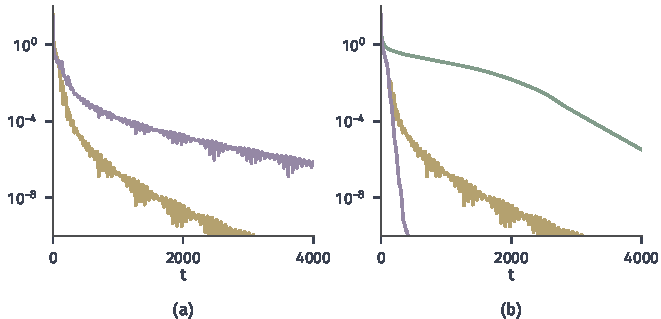
\includegraphics[width=112mm]{figures/05-optimization/03-nonsmooth-optimization/matplotlib/ns-residual-restart/figure.pdf}
  \caption{FISTA的残差与重启，问题与图~\ref{fig:ns-ista-fista-rates}相同（半对数坐标）。(a)黄线是目标差，紫线是$\bm{x}^{(t)}$处的映射残差范数，两者都不单调。(b)绿线是ISTA，黄线是FISTA，紫线是带函数值重启的FISTA。}
  \label{fig:ns-residual-restart}
\end{BookInlineFigure}

\paragraph{成本对比}
比较ISTA和FISTA时，把一次迭代的成本拆开。

\begin{BookInlineTable}
  \centering
  \small
  \begin{tabular}{@{}lll@{}}
    \toprule
     & ISTA & FISTA\\
    \midrule
    每步梯度 & $1$次，在$\bm{x}^{(t)}$ & $1$次，在$\bm{y}^{(t)}$\\
    每步邻近映射 & $1$次 & $1$次\\
    额外存储 & 无 & $\bm{x}^{(t-1)}$与$\bm{y}^{(t)}$\\
    回溯 & 每次试探增加$1$次邻近、$1$次$f$ & 同左，试探点是$\bm{y}^{(t)}$\\
    目标值单调 & 是 & 否\\
    目标差界 & $O(1/T)$ & $O(1/T^2)$\\
    非凸$f$ & 残差界式~\eqref{eq:ns-nonconvex-residual} & 无此保证\\
    \bottomrule
  \end{tabular}
  \caption{ISTA与FISTA的成本和保证。计算函数值用于重启或停止时，FISTA每轮还要加上一次$F$的计算。}
  \label{tab:ns-ista-fista}
\end{BookInlineTable}

对Lasso，一次梯度$\bm{A}^\top(\bm{A}\bm{x}-\bm{b})$是两次矩阵向量乘，一次软阈值只要$O(n)$。主要成本在矩阵向量乘，所以“迭代次数”可以当作比较的单位。当邻近映射本身要迭代时，这个单位就不合适了，比较必须按总的基本运算数，见表~\ref{tab:ns-ista-fista}。

\section{光滑化}
\label{sec:ns-smoothing}

邻近方法要求非光滑项的邻近映射便宜。有限个仿射函数的最大值常常做不到这一点：它的邻近子问题本身是一个二次规划。于是要问：能否把尖点磨圆，得到一个光滑的替代目标，再调用第~\ref{chap:first-order-methods}章的方法，并算清这样做对原问题到底造成多大误差？

光滑化改变的是目标，第~\ref{chap:first-order-methods}章的Nesterov加速改变的是迭代规则，这是两件独立的事，后面会把它们配合使用。从本节起，$\mu>0$表示平滑参数，$\mu$越小替代目标越接近原目标。

\subsection{Huber逼近}
\label{sec:ns-huber}

最简单的尖点是$\lvert x\rvert$的原点。把原点两侧长度为$\mu$的两段折线换成一段抛物线，外面保持直线，就把尖点磨掉了。外面的直线不能是$\lvert x\rvert$本身，否则接不上，要向下平移一段。设抛物线是$x^2/(2\mu)$，外侧是$\lvert x\rvert-c$，在接点$x=\mu$处要求函数值和一阶导数都匹配。

一阶导数：抛物线的导数是$x/\mu$，在$x=\mu$处等于$1$，正好等于外侧直线的斜率，这是抛物线取系数$1/(2\mu)$的原因。

函数值：抛物线在接点的值是$\mu/2$，要求$\mu-c=\mu/2$，所以$c=\mu/2$。

这样得到\term{Huber函数}（Huber function）\scite{huber1964}
\begin{equation}
 h_\mu(x)=\begin{cases}
 \dfrac{x^2}{2\mu},&\lvert x\rvert\leq\mu,\\
 \lvert x\rvert-\dfrac{\mu}{2},&\lvert x\rvert>\mu.
 \end{cases}
 \label{eq:ns-huber}
\end{equation}

下面的性质说明它是一个可控的替代。

\begin{theorem}[Huber逼近的性质]
\label{thm:ns-huber}
对任意$\mu>0$，$h_\mu$是连续可微的凸函数，并且
\begin{gather}
 0\leq\lvert x\rvert-h_\mu(x)\leq\frac{\mu}{2},\label{eq:ns-huber-gap}\\
 h_\mu'(x)=\min\Bigl\{\max\Bigl\{\frac{x}{\mu},\,-1\Bigr\},\,1\Bigr\},\qquad
 \lvert h_\mu'(x)-h_\mu'(y)\rvert\leq\frac{1}{\mu}\lvert x-y\rvert.\label{eq:ns-huber-grad}
\end{gather}
\end{theorem}

\begin{proof}
由接点匹配，$h_\mu$在$\pm\mu$处连续可微，其余点是二次函数或线性函数，也可微，导数就是式~\eqref{eq:ns-huber-grad}。这个导数是$x/\mu$截断到$[-1,1]$，它单调不减（所以$h_\mu$凸）。截断不增大距离，而$x/\mu$的Lipschitz常数是$1/\mu$，所以导数$1/\mu$-Lipschitz。

偏差只需看$x\geq0$。外侧$\lvert x\rvert-h_\mu(x)=\mu/2$。内侧令$e(x)=x-x^2/(2\mu)$，$e(0)=0$，$e'(x)=1-x/\mu\geq0$，所以$e$从$0$单调增到$e(\mu)=\mu/2$。
\end{proof}

图~\ref{fig:ns-huber}画出两个$\mu$。(a)中$h_\mu$从下方逼近$\lvert x\rvert$，$\mu$减半时差也减半。(b)中$\lvert x\rvert$的导数在原点跳变，$h_\mu'$用一段斜率$1/\mu$的直线走完这段跳变。$\mu$减半，过渡段的斜率加倍，这就是梯度Lipschitz常数$1/\mu$的来源。

\begin{BookInlineFigure}
  \centering
  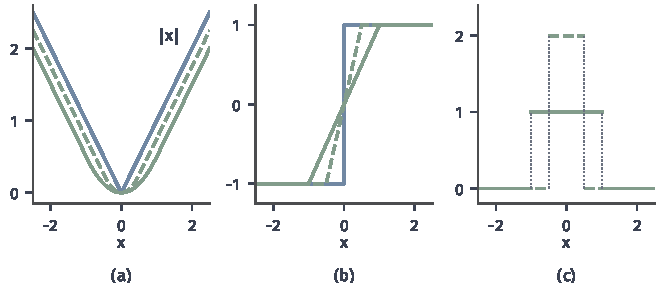
\includegraphics[width=112mm]{figures/05-optimization/03-nonsmooth-optimization/matplotlib/ns-huber/figure.pdf}
  \caption{Huber函数。蓝线是$\lvert x\rvert$及其导数，绿色实线和虚线分别是$\mu=1$和$\mu=\tfrac12$的$h_\mu$。(a)函数值，$h_\mu$在外侧与$\lvert x\rvert$平行。(b)一阶导数，连续但有拐点。(c)二阶导数，在接点$\pm\mu$处跳变，所以$h_\mu$在这些点不是二阶可微的。}
  \label{fig:ns-huber}
\end{BookInlineFigure}

要留意图~\ref{fig:ns-huber}(c)。$h_\mu$的二阶导数在$\lvert x\rvert<\mu$处是$1/\mu$，在外面是$0$，在接点上不存在。所以$h_\mu$的梯度Lipschitz，但不是处处二阶可微。第~\ref{chap:smooth-foundations}章的一阶方法只需要前者，可以直接用；第~\ref{chap:second-order-methods}章的牛顿法在接点附近没有定义好的Hessian，要专门处理。

\subsection{Moreau包络}
\label{sec:ns-moreau}

Huber函数的抛物线从何而来？它其实是第~\ref{sec:ns-proximal}节的邻近子问题的副产品：邻近映射取的是最小点，如果取最优值，就得到一个新函数。

\begin{definition}[Moreau包络]
\label{def:ns-moreau}
设$f$是适当、下半连续的凸函数，$\mu>0$。称
\begin{equation}
 M_{\mu f}(\bm{x})=\min_{\bm{y}}\Bigl\{f(\bm{y})+\frac{1}{2\mu}\lVert\bm{y}-\bm{x}\rVert_2^2\Bigr\}
 \label{eq:ns-moreau}
\end{equation}
为$f$的\term{Moreau包络}（Moreau envelope）。
\end{definition}

由定理~\ref{thm:ns-prox}，最小值在唯一的$\bm{p}=\operatorname{prox}_{\mu f}(\bm{x})$处取到，所以$M_{\mu f}$处处有限。

对$f=\lvert\cdot\rvert$用软阈值计算。若$\lvert x\rvert\leq\mu$，$p=0$，结果是$x^2/(2\mu)$。若$\lvert x\rvert>\mu$，$p=x-\mu\operatorname{sign}(x)$，$\lvert p\rvert=\lvert x\rvert-\mu$，距离项是$\mu/2$，结果是$\lvert x\rvert-\mu/2$。两种情形合起来正是式~\eqref{eq:ns-huber}：
\begin{equation}
 M_{\mu\lvert\cdot\rvert}=h_\mu.
 \label{eq:ns-moreau-huber}
\end{equation}

这个包络的图景是：把一个以$\bm{x}$为顶点的小抛物线碗从下往上抬，碰到$f$时碗顶的高度就是$M_{\mu f}(\bm{x})$。图~\ref{fig:ns-moreau-envelope}(a)画出了三段折线的包络，折点都被抛物线磨圆。

\begin{theorem}[Moreau包络的光滑性与最小点]
\label{thm:ns-moreau}
设$f$是适当、下半连续的凸函数，$\mu>0$。则$M_{\mu f}$是凸函数，处处可微，且
\begin{equation}
 \nabla M_{\mu f}(\bm{x})=\frac{\bm{x}-\operatorname{prox}_{\mu f}(\bm{x})}{\mu}.
 \label{eq:ns-moreau-grad}
\end{equation}
梯度是$1/\mu$-Lipschitz的。此外$M_{\mu f}\leq f$，并且$M_{\mu f}$与$f$有相同的最小值和相同的最小点集合。
\end{theorem}

\begin{proof}
记$\bm{p}=\operatorname{prox}_{\mu f}(\bm{x})$，$\bm{s}=(\bm{x}-\bm{p})/\mu$，由式~\eqref{eq:ns-prox-characterization}有$\bm{s}\in\partial f(\bm{p})$。任取$\bm{y}$，记$\bm{q}=\operatorname{prox}_{\mu f}(\bm{y})$。

上界。把$\bm{p}$作为$\bm{y}$处子问题的试探点，
\[
 M_{\mu f}(\bm{y})\leq f(\bm{p})+\frac{1}{2\mu}\lVert\bm{p}-\bm{y}\rVert_2^2=M_{\mu f}(\bm{x})+\langle\bm{s},\bm{y}-\bm{x}\rangle+\frac{1}{2\mu}\lVert\bm{y}-\bm{x}\rVert_2^2.
\]
第二个等号是把$\bm{p}-\bm{y}=(\bm{p}-\bm{x})+(\bm{x}-\bm{y})$展开，并用$\bm{p}-\bm{x}=-\mu\bm{s}$。

下界。由$\bm{s}\in\partial f(\bm{p})$，
\[
 f(\bm{q})\geq f(\bm{p})+\langle\bm{s},\bm{q}-\bm{p}\rangle,
\]
于是
\[
 M_{\mu f}(\bm{y})-M_{\mu f}(\bm{x})\geq\langle\bm{s},\bm{q}-\bm{p}\rangle+\frac{1}{2\mu}\Bigl(\lVert\bm{q}-\bm{y}\rVert_2^2-\lVert\bm{p}-\bm{x}\rVert_2^2\Bigr).
\]

记$\bm{a}=\bm{q}-\bm{y}$，$\bm{b}=\bm{p}-\bm{x}=-\mu\bm{s}$，再用恒等式
\[
 \lVert\bm{a}\rVert_2^2-\lVert\bm{b}\rVert_2^2=\lVert\bm{a}-\bm{b}\rVert_2^2+2\langle\bm{a}-\bm{b},\bm{b}\rangle,
\]
右端化为
\[
 \langle\bm{s},\bm{y}-\bm{x}\rangle+\frac{1}{2\mu}\lVert\bm{a}-\bm{b}\rVert_2^2\geq\langle\bm{s},\bm{y}-\bm{x}\rangle.
\]

上下界合起来，
\[
 0\leq M_{\mu f}(\bm{y})-M_{\mu f}(\bm{x})-\langle\bm{s},\bm{y}-\bm{x}\rangle\leq\frac{1}{2\mu}\lVert\bm{y}-\bm{x}\rVert_2^2.
\]
所以$M_{\mu f}$在$\bm{x}$处可微，梯度为$\bm{s}$。下界对所有$\bm{x}$成立，说明处处存在次梯度，因而是凸函数。

Lipschitz性。记$\bm{u}=\bm{x}-\bm{y}$，$\bm{w}=\bm{p}-\bm{q}$，由式~\eqref{eq:ns-firm-nonexpansive}得$\lVert\bm{w}\rVert_2^2$不超过$\langle\bm{u},\bm{w}\rangle$，所以
\[
 \lVert\bm{u}-\bm{w}\rVert_2^2=\lVert\bm{u}\rVert_2^2-2\langle\bm{u},\bm{w}\rangle+\lVert\bm{w}\rVert_2^2\leq\lVert\bm{u}\rVert_2^2-\lVert\bm{w}\rVert_2^2\leq\lVert\bm{u}\rVert_2^2.
\]
梯度之差是$(\bm{u}-\bm{w})/\mu$，范数不超过$\lVert\bm{u}\rVert_2/\mu$。

最小点。在式~\eqref{eq:ns-moreau}中取$\bm{y}=\bm{x}$得$M_{\mu f}\leq f$。$\bm{x}$是$M_{\mu f}$的最小点，当且仅当梯度为零，当且仅当$\bm{x}=\operatorname{prox}_{\mu f}(\bm{x})$，由式~\eqref{eq:ns-prox-characterization}当且仅当$\bm{0}\in\partial f(\bm{x})$。此时距离项为零，$M_{\mu f}(\bm{x})=f(\bm{x})$，所以最小值相同。
\end{proof}

对$\lvert x\rvert$验证式~\eqref{eq:ns-moreau-grad}。$x=2$，$\mu=1$时$p=1$，公式给出$(2-1)/1=1$，这就是Huber函数在外侧的斜率。$x=0.6$时$p=0$，公式给出$0.6$，与$h_1'(0.6)=0.6$一致。

\paragraph{平滑一项不等于保持解}
定理说整个凸目标的包络与原函数有相同的最小点。但实用上想平滑的通常只是复合目标的一项。这时最小点一般会变。

取$F(x)=\tfrac12(x-\tfrac12)^2+\lvert x\rvert$。在$x=0$处$F$的次微分是$-\tfrac12+[-1,1]$，包含零，所以$x^\star=0$。只把$\lvert x\rvert$换成包络$h_1$，得到光滑目标$F_1(x)=\tfrac12(x-\tfrac12)^2+h_1(x)$，在$\lvert x\rvert\leq1$上令导数为零：
\[
 x-\frac12+x=0,\qquad x=\frac14.
\]

原问题的解是$0$，这个替代的解是$\tfrac14$。图~\ref{fig:ns-moreau-envelope}(b)显示了这一点。代入原目标，$F(\tfrac14)=\tfrac{9}{32}\approx0.281$，比$F^\star=\tfrac18$高，$\tfrac14$不再有“稀疏”的零分量。

\begin{BookInlineFigure}
  \centering
  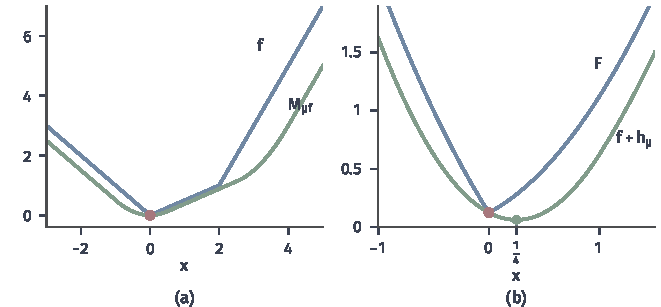
\includegraphics[width=112mm]{figures/05-optimization/03-nonsmooth-optimization/matplotlib/ns-moreau-envelope/figure.pdf}
  \caption{Moreau包络（$\mu=1$）。(a)三段折线$f$（蓝）与它的包络（绿），最小点相同（红点）。(b)$F(x)=\tfrac12(x-\tfrac12)^2+\lvert x\rvert$（蓝）的最小点是$0$（红点），只平滑绝对值项后，绿色替代目标的最小点移到$\tfrac14$（绿点）。}
  \label{fig:ns-moreau-envelope}
\end{BookInlineFigure}

求包络的梯度~\eqref{eq:ns-moreau-grad}要算一次邻近映射。所以包络不能绕开邻近映射：当$\operatorname{prox}$不便宜时，这条路同样走不通。这正是下面的方法要解决的问题。

\subsection{Nesterov平滑}
\label{sec:ns-nesterov-smoothing}

许多非光滑函数天然写成最大值，比如分段线性函数和$\ell_1$范数。最大值函数的梯度在活跃分支切换时跳变。Nesterov平滑的想法是让这种切换变得连续，方法是在最大化问题的变量上加入一点强凸惩罚，使每个$\bm{x}$对应唯一的内层最优点，而这个最优点随$\bm{x}$连续变化。

\subsubsection{最大值表示的正则化}
\label{sec:ns-max-regularization}

设目标有最大值结构：$\bm{A}\in\mathbb{R}^{p\times n}$，$\bm{Q}\subset\mathbb{R}^p$是非空紧凸集，$\phi$是$\bm{Q}$上的连续凸函数，
\begin{equation}
 f(\bm{x})=\max_{\bm{u}\in\bm{Q}}\bigl\{\langle\bm{A}\bm{x},\bm{u}\rangle-\phi(\bm{u})\bigr\}.
 \label{eq:ns-max-form}
\end{equation}

例如$\lvert x\rvert=\max_{\lvert u\rvert\leq1}xu$，最优的$u$是$\operatorname{sign}(x)$，在$x=0$处从$-1$跳到$1$，这就是梯度的跳变。

在$\bm{u}$的空间选一个范数$\lVert\cdot\rVert_{\bm{Q}}$。设$d:\bm{Q}\to\mathbb{R}$连续，$\sigma$-强凸（对这个范数），且$\min_{\bm{Q}}d=0$。记$D=\max_{\bm{Q}}d$，矩阵的范数
\[
 \lVert\bm{A}\rVert=\max\bigl\{\langle\bm{A}\bm{x},\bm{u}\rangle:\ \lVert\bm{x}\rVert_2\leq1,\ \lVert\bm{u}\rVert_{\bm{Q}}\leq1\bigr\}.
\]

这里的$\sigma$-强凸是指对$\bm{u},\bm{v}\in\bm{Q}$，$\theta\in[0,1]$，
\begin{equation}
 d\bigl(\theta\bm{u}+(1-\theta)\bm{v}\bigr)\leq\theta d(\bm{u})+(1-\theta)d(\bm{v})-\frac{\sigma}{2}\theta(1-\theta)\lVert\bm{u}-\bm{v}\rVert_{\bm{Q}}^2.
 \label{eq:ns-sigma-strong}
\end{equation}
在最大化式里减去$\mu d$，定义\term{Nesterov平滑}（Nesterov smoothing）
\begin{equation}
 f_\mu(\bm{x})=\max_{\bm{u}\in\bm{Q}}\bigl\{\langle\bm{A}\bm{x},\bm{u}\rangle-\phi(\bm{u})-\mu d(\bm{u})\bigr\}.
 \label{eq:ns-nesterov}
\end{equation}

\begin{theorem}[Nesterov平滑的性质]
\label{thm:ns-nesterov}
在上述条件下，式~\eqref{eq:ns-nesterov}对每个$\bm{x}$有唯一的最大点，记作$\bm{u}_\mu(\bm{x})$。函数$f_\mu$凸且可微，并且
\begin{gather}
 \nabla f_\mu(\bm{x})=\bm{A}^\top\bm{u}_\mu(\bm{x}),\label{eq:ns-nesterov-grad}\\
 f_\mu(\bm{x})\leq f(\bm{x})\leq f_\mu(\bm{x})+\mu D,\label{eq:ns-nesterov-gap}\\
 \lVert\nabla f_\mu(\bm{x})-\nabla f_\mu(\bm{y})\rVert_2\leq\frac{\lVert\bm{A}\rVert^2}{\mu\sigma}\lVert\bm{x}-\bm{y}\rVert_2.\label{eq:ns-nesterov-lip}
\end{gather}
\end{theorem}

\begin{proof}
记式~\eqref{eq:ns-nesterov}中大括号内的函数为$\Psi_{\bm{x}}(\bm{u})$。$\phi$是凸的，$\mu d$是$\mu\sigma$-强凸的，所以$\Psi_{\bm{x}}$是$\mu\sigma$-强凹的连续函数，在紧凸集上有唯一的最大点。

强凹性给出最大点处的二次间隙。设$\bm{u}_1$是最大点，对任意$\bm{u}\in\bm{Q}$和$\theta\in(0,1)$，令$\bm{w}=\theta\bm{u}+(1-\theta)\bm{u}_1\in\bm{Q}$，
\[
 \Psi_{\bm{x}}(\bm{u}_1)\geq\Psi_{\bm{x}}(\bm{w})\geq\theta\Psi_{\bm{x}}(\bm{u})+(1-\theta)\Psi_{\bm{x}}(\bm{u}_1)+\frac{\mu\sigma}{2}\theta(1-\theta)\lVert\bm{u}-\bm{u}_1\rVert_{\bm{Q}}^2.
\]

整理后除以$\theta$，再令$\theta\to0$，得到
\begin{equation}
 \Psi_{\bm{x}}(\bm{u})\leq\Psi_{\bm{x}}(\bm{u}_1)-\frac{\mu\sigma}{2}\lVert\bm{u}-\bm{u}_1\rVert_{\bm{Q}}^2.
 \label{eq:ns-strong-concave-gap}
\end{equation}

Lipschitz估计。对$\bm{x}_1,\bm{x}_2$，记$\bm{u}_i=\bm{u}_\mu(\bm{x}_i)$。式~\eqref{eq:ns-strong-concave-gap}两次使用后相加，$\phi$和$d$的项消去，得到
\[
 \mu\sigma\lVert\bm{u}_1-\bm{u}_2\rVert_{\bm{Q}}^2\leq\langle\bm{A}(\bm{x}_1-\bm{x}_2),\bm{u}_1-\bm{u}_2\rangle\leq\lVert\bm{A}\rVert\,\lVert\bm{x}_1-\bm{x}_2\rVert_2\,\lVert\bm{u}_1-\bm{u}_2\rVert_{\bm{Q}}.
\]

约去一个$\lVert\bm{u}_1-\bm{u}_2\rVert_{\bm{Q}}$，得到
\[
 \lVert\bm{u}_1-\bm{u}_2\rVert_{\bm{Q}}\leq\frac{\lVert\bm{A}\rVert}{\mu\sigma}\lVert\bm{x}_1-\bm{x}_2\rVert_2.
\]

梯度公式。$f_\mu$是一族仿射函数的上确界，所以是凸的。取$\bm{u}=\bm{u}_\mu(\bm{x})$，$\bm{u}'=\bm{u}_\mu(\bm{y})$，一方面
\[
 f_\mu(\bm{y})\geq\Psi_{\bm{y}}(\bm{u})=f_\mu(\bm{x})+\langle\bm{A}^\top\bm{u},\bm{y}-\bm{x}\rangle.
\]

另一方面，由$\Psi_{\bm{x}}(\bm{u}')\leq f_\mu(\bm{x})$，
\[
 f_\mu(\bm{y})=\Psi_{\bm{y}}(\bm{u}')\leq f_\mu(\bm{x})+\langle\bm{A}^\top\bm{u},\bm{y}-\bm{x}\rangle+\langle\bm{A}(\bm{y}-\bm{x}),\bm{u}'-\bm{u}\rangle.
\]
由上一段的估计，最后一项不超过$\lVert\bm{A}\rVert^2\lVert\bm{y}-\bm{x}\rVert_2^2/(\mu\sigma)$，是二阶小量，所以$f_\mu$可微，梯度是$\bm{A}^\top\bm{u}$。

式~\eqref{eq:ns-nesterov-lip}由上面的估计和下面的范数关系得到：
\[
 \lVert\bm{A}^\top(\bm{u}_1-\bm{u}_2)\rVert_2\leq\lVert\bm{A}\rVert\,\lVert\bm{u}_1-\bm{u}_2\rVert_{\bm{Q}}.
\]

偏差。由$0\leq d\leq D$，对每个$\bm{u}$有
\[
 \langle\bm{A}\bm{x},\bm{u}\rangle-\phi(\bm{u})-\mu D\leq\Psi_{\bm{x}}(\bm{u})\leq\langle\bm{A}\bm{x},\bm{u}\rangle-\phi(\bm{u}).
\]
对$\bm{u}$取最大，就是式~\eqref{eq:ns-nesterov-gap}。
\end{proof}

每个条件的作用都清楚：紧性使$D$有限，从而偏差有限；强凸使内层解唯一且随$\bm{x}$连续变化，梯度跳变由此被抹平；$\min d=0$让偏差是单侧的。$\mu$变小时偏差$\mu D$变小，Lipschitz常数$\lVert\bm{A}\rVert^2/(\mu\sigma)$变大，后面就是要权衡这两者。

用菱形目标算一遍。写成$\bm{A}=\operatorname{diag}(1,2)$，$\bm{Q}=[-1,1]^2$，$\phi=0$，$d(\bm{u})=\tfrac12\lVert\bm{u}\rVert_2^2$，$\sigma=1$，范数取欧氏范数。此时$D=1$，$\lVert\bm{A}\rVert=2$。内层问题按坐标分开，解是把$(\bm{A}\bm{x})_i/\mu$截断到$[-1,1]$，把解代回，得到
\[
 f_\mu(\bm{x})=h_\mu(x_1)+h_\mu(2x_2),\qquad\nabla f_\mu(\bm{x})=\bm{A}^\top\bm{u}_\mu(\bm{x}).
\]

结果是两个Huber函数之和，第二项的二阶导数最大为$4/\mu$，正好是$\lVert\bm{A}\rVert^2/(\mu\sigma)$。在$\bm{x}=(1,0)$，$\mu=1$处，
\[
 \bm{u}_1=(1,0),\qquad f_1(\bm{x})=\frac12,\qquad f(\bm{x})-f_1(\bm{x})=\frac12\leq\mu D=1.
\]

内层求解的成本决定这个方法是否划算。本例内层是逐坐标截断，$O(n)$；$\bm{Q}$是单纯形且$d$取下面的负熵时也是闭式解。若$\bm{Q}$或$\phi$没有这样的结构，每次读梯度都要解一个内层优化，只能得到近似的$\bm{u}_\mu$，这时梯度带有误差，上面的保证需要重新计入这个误差。

\subsubsection{对数和指数平滑}
\label{sec:ns-log-sum-exp}

最常用的实例是有限个仿射函数的最大值，也就是开头提到的邻近映射不便宜的情形。设$\ell_i(\bm{x})=\langle\bm{a}_i,\bm{x}\rangle+b_i$，$i=1,\ldots,m$，这里$m$是分支个数。

把“选一个最大的分支”写成单纯形$\Delta_m=\{\bm{u}\geq\bm{0}:\sum_iu_i=1\}$上的线性最大化，权重集中在最大的分支上时取到最大值：
\[
 f(\bm{x})=\max_i\ell_i(\bm{x})=\max_{\bm{u}\in\Delta_m}\sum_{i=1}^mu_i\ell_i(\bm{x}).
\]

这符合式~\eqref{eq:ns-max-form}，$\bm{A}$的第$i$行是$\bm{a}_i^\top$，$\phi(\bm{u})=-\sum_iu_ib_i$。选择归一化的\term{负熵}（negative entropy）作为$d$：
\[
 d(\bm{u})=\sum_{i=1}^mu_i\ln u_i+\ln m.
\]

$d$的最小值$0$在均匀分布处取到，最大值$\ln m$在顶点处取到，所以$D=\ln m$。

内层问题是
\[
 \max_{\bm{u}\in\Delta_m}\ \sum_iu_i\ell_i-\mu\sum_iu_i\ln u_i-\mu\ln m.
\]

对约束$\sum_iu_i=1$引入乘子，令对$u_i$的偏导数为零，得$\ell_i-\mu(\ln u_i+1)+\nu=0$，也就是$u_i\propto\exp(\ell_i/\mu)$。解是softmax权重：
\begin{equation}
 p_i(\bm{x})=\frac{\exp(\ell_i(\bm{x})/\mu)}{\sum_{k=1}^m\exp(\ell_k(\bm{x})/\mu)}.
 \label{eq:ns-softmax}
\end{equation}

记分母为$Z$，由$\ln p_i=\ell_i/\mu-\ln Z$，代回内层目标，$\ell_i$的项消去，得到
\begin{equation}
 f_\mu(\bm{x})=\mu\ln\frac{1}{m}\sum_{i=1}^m\exp\Bigl(\frac{\ell_i(\bm{x})}{\mu}\Bigr).
 \label{eq:ns-lse-lower}
\end{equation}

不做归一化的版本是最常见的\term{对数和指数函数}（log-sum-exp function）
\begin{equation}
 \varphi_\mu(\bm{x})=\mu\ln\sum_{i=1}^m\exp\Bigl(\frac{\ell_i(\bm{x})}{\mu}\Bigr)=f_\mu(\bm{x})+\mu\ln m.
 \label{eq:ns-lse-upper}
\end{equation}

两者只差常数$\mu\ln m$，梯度相同。由式~\eqref{eq:ns-nesterov-gap}，前者从下方逼近，后者从上方逼近：
\begin{equation}
 f-\mu\ln m\leq f_\mu\leq f\leq\varphi_\mu\leq f+\mu\ln m.
 \label{eq:ns-lse-gap}
\end{equation}

上方这一半可以直接看出来。把$\exp(f/\mu)$提到求和号外，求和的每一项不超过$1$，最大的一项等于$1$，所以和在$1$到$m$之间。

对$\bm{x}$求导，梯度是softmax加权的分支斜率：
\begin{equation}
 \nabla f_\mu(\bm{x})=\sum_{i=1}^mp_i(\bm{x})\,\bm{a}_i.
 \label{eq:ns-lse-grad}
\end{equation}

再求一次导，Hessian是斜率的协方差除以$\mu$：
\[
 \nabla^2f_\mu=\frac1\mu\Bigl(\sum_ip_i\bm{a}_i\bm{a}_i^\top-\bar{\bm{a}}\bar{\bm{a}}^\top\Bigr),\qquad\bar{\bm{a}}=\sum_ip_i\bm{a}_i.
\]

对单位向量$\bm{v}$，$\bm{v}^\top\nabla^2f_\mu\bm{v}$是取值$\langle\bm{a}_i,\bm{v}\rangle$的随机变量的方差除以$\mu$，不超过$\max_i\lVert\bm{a}_i\rVert_2^2/\mu$。所以
\begin{equation}
 L_\mu=\frac{\max_i\lVert\bm{a}_i\rVert_2^2}{\mu}.
 \label{eq:ns-lse-lipschitz}
\end{equation}

这也符合定理~\ref{thm:ns-nesterov}：负熵在$\Delta_m$上对$\ell_1$范数是$1$-强凸的（Pinsker不等式），相应的$\lVert\bm{A}\rVert=\max_i\lVert\bm{a}_i\rVert_2$，式~\eqref{eq:ns-lse-lipschitz}正是$\lVert\bm{A}\rVert^2/(\mu\sigma)$。这里取$\ell_1$范数，比欧氏范数给出的$\lVert\bm{A}\rVert_2^2/\mu$更小，这就是在定理中允许一般范数的原因。

用三段折线核对。$\mu=1$时，$x=0$处三支的值是$0,0,-3$，权重正比于$1,1,e^{-3}$，也就是
\[
 \bm{p}\approx(0.488,\,0.488,\,0.024).
\]

导数是权重与斜率的内积：
\[
 f_1'(0)\approx0.488\cdot(-1)+0.488\cdot\tfrac12+0.024\cdot2\approx-0.195.
\]

原函数在$x=0$的次微分是$[-1,\tfrac12]$，这个数落在其中。图~\ref{fig:ns-inner-maximizer}(a)画出了$\mu=0.2$时权重随$x$的变化：原本的分支切换被抹成了平滑的过渡。图~\ref{fig:ns-inner-maximizer}(b)中，导数的跳变被抹平，$\mu$越小越接近原来的台阶。

\begin{BookInlineFigure}
  \centering
  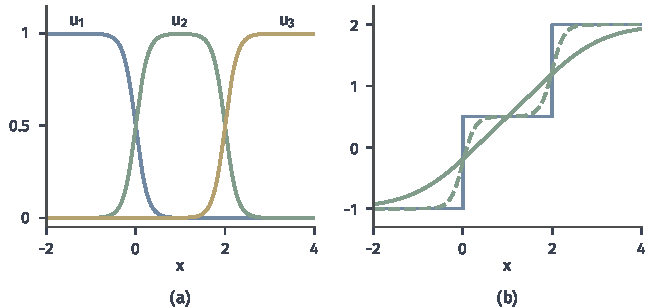
\includegraphics[width=112mm]{figures/05-optimization/03-nonsmooth-optimization/matplotlib/ns-inner-maximizer/figure.pdf}
  \caption{三段折线的熵平滑。(a)$\mu=0.2$时的内层最优权重$u_i=p_i(x)$，蓝、绿、黄分别对应斜率$-1,\tfrac12,2$的分支。(b)蓝线是原函数的次微分（台阶），绿色虚线和实线分别是$\mu=0.2$和$\mu=1$的$f_\mu'$，由权重加权平均得到。}
  \label{fig:ns-inner-maximizer}
\end{BookInlineFigure}

\paragraph{与Huber比较}
$\lvert x\rvert=\max\{x,-x\}$有两个分支，$m=2$，把两种平滑写出来：
\[
 \varphi_\mu(x)=\mu\ln\bigl(e^{x/\mu}+e^{-x/\mu}\bigr),\qquad f_\mu(x)=\mu\ln\cosh\frac{x}{\mu}.
\]

两者的导数都是$\tanh(x/\mu)$，二阶导数都不超过$1/\mu$，这与Huber函数的$1/\mu$相同。差别在形状和偏差，图~\ref{fig:ns-log-sum-exp}对比了三者（$\mu=\tfrac12$）。

\begin{BookInlineFigure}
  \centering
  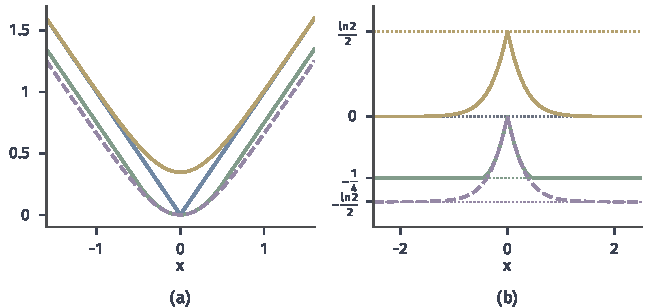
\includegraphics[width=112mm]{figures/05-optimization/03-nonsmooth-optimization/matplotlib/ns-log-sum-exp/figure.pdf}
  \caption{$\lvert x\rvert$（蓝）的三种平滑，$\mu=\tfrac12$：Huber（绿）、未平移的对数和指数函数$\varphi_\mu$（黄）、归一化版本$f_\mu$（紫色虚线）。(a)函数值。(b)替代函数减$\lvert x\rvert$的差，点线标出各自的极限或最大偏差$-\mu/2$、$\pm\mu\ln2$。}
  \label{fig:ns-log-sum-exp}
\end{BookInlineFigure}

Huber函数在$\pm\mu$外与$\lvert x\rvert$只差一个常数，偏差$\mu/2$；对数和指数函数的过渡是指数式的，走不到精确的斜率$\pm1$，偏差最大是$\mu\ln2\approx0.693\mu$。上方的$\varphi_\mu$偏差在原点最大，向外趋于零；下方的$f_\mu$在原点无偏差，向外趋于$\mu\ln2$。表~\ref{tab:ns-smoothers}汇总了这些差别。

\begin{BookInlineTable}
  \centering
  \small
  \begin{tabular}{@{}llll@{}}
    \toprule
     & Huber & 上方$\varphi_\mu$ & 下方$f_\mu$\\
    \midrule
    构造 & Moreau包络 & 负熵，不平移 & 负熵，归一化\\
    偏差范围 & $[0,\mu/2]$ & $[0,\mu\ln2]$ & $[0,\mu\ln2]$\\
    相对原函数 & 下方 & 上方 & 下方\\
    梯度Lipschitz & $1/\mu$ & $1/\mu$ & $1/\mu$\\
    二阶可微 & 否 & 是 & 是\\
    推广到$m$个分支 & 需要邻近映射 & 显式，偏差$\mu\ln m$ & 显式，偏差$\mu\ln m$\\
    \bottomrule
  \end{tabular}
  \caption{$\lvert x\rvert$的三种光滑替代。}
  \label{tab:ns-smoothers}
\end{BookInlineTable}

\subsection{平滑偏差与求解精度}
\label{sec:ns-smoothing-accuracy}

光滑化引入了两种误差：替代目标与原目标的差别，以及替代问题没有求准的部分。给定原问题的精度要求，这两者要联合分配。

\paragraph{误差分解}
设$F$是原目标，光滑替代$F_\mu$满足统一偏差界$F_\mu\leq F\leq F_\mu+\mu D$，例如式~\eqref{eq:ns-nesterov-gap}。对任意$\hat{\bm{x}}$和$F$的最小点$\bm{x}^\star$，由$F(\hat{\bm{x}})\leq F_\mu(\hat{\bm{x}})+\mu D$和$F_\mu(\bm{x}^\star)\leq F^\star$，
\begin{equation}
 F(\hat{\bm{x}})-F^\star\leq\bigl(F_\mu(\hat{\bm{x}})-F_\mu(\bm{x}^\star)\bigr)+\mu D.
 \label{eq:ns-smoothing-split}
\end{equation}

右端第一项是求解误差，可以靠多走几步减小；第二项是平滑偏差，无论替代问题解得多准都留在那里。这里的比较点取$\bm{x}^\star$而不是$F_\mu$的最小点，因此第一项可以直接用定理~\ref{thm:ns-fista-rate}的任意比较点版本控制。上方逼近的$\varphi_\mu$与$f_\mu$只差常数，上式同样适用。

图~\ref{fig:ns-smoothing-budget}(a)在$\mathbb{R}^2$上$7$个分支的问题上显示了这件事：固定$\mu$跑加速方法，原目标差最终停在由$\mu\ln m$决定的平台上；$\mu$越小，平台越低，到达平台需要的步数越多。

\begin{BookInlineFigure}
  \centering
  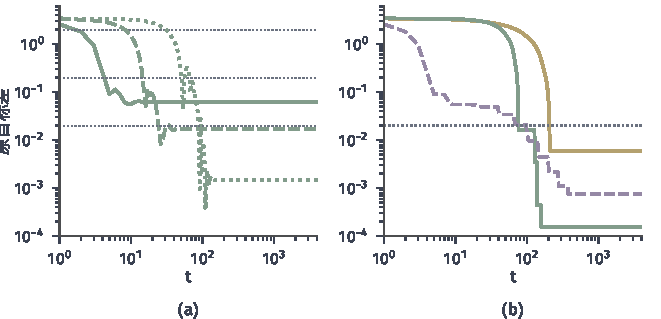
\includegraphics[width=112mm]{figures/05-optimization/03-nonsmooth-optimization/matplotlib/ns-smoothing-budget/figure.pdf}
  \caption{偏差与求解精度（双对数坐标）。目标是平面上$7$个等分方向的单位斜率分支的最大值，$\bm{x}^{(0)}=(3,2)$，用熵平滑配合Nesterov加速，$\alpha=1/L_\mu=\mu$。(a)绿色实线、虚线、点线分别是$\mu=1,0.1,0.01$时原目标差，灰色点线是偏差上界$\mu\ln7$。(b)目标精度$\varepsilon=0.02$（灰色点线）：黄线是固定步长$\alpha=\varepsilon$的次梯度法的最好值，绿线是取$\mu=\varepsilon/(2\ln7)$的平滑加速法，紫色虚线是$\mu$逐阶段减半、同步更新步长的方案。}
  \label{fig:ns-smoothing-budget}
\end{BookInlineFigure}

\paragraph{总成本}
下面的定理把偏差、光滑常数、加速方法合在一起。

\begin{theorem}[平滑加速法的总成本]
\label{thm:ns-smoothing-cost}
设$F=\psi+f$，$\psi$是凸函数且梯度$L_\psi$-Lipschitz连续（可以为零），$f$具有式~\eqref{eq:ns-max-form}的结构，$F$存在最小点$\bm{x}^\star$，$\lVert\bm{x}^{(0)}-\bm{x}^\star\rVert_2\leq R$。对$F_\mu=\psi+f_\mu$运行式~\eqref{eq:ns-fista}（$r=0$），步长$\alpha=1/L_\mu$，$L_\mu=L_\psi+\lVert\bm{A}\rVert^2/(\mu\sigma)$。给定$\varepsilon>0$，取
\begin{equation}
 \mu=\frac{\varepsilon}{2D},
 \label{eq:ns-mu-choice}
\end{equation}
则当
\begin{equation}
 T+1\geq2R\sqrt{\frac{L_\psi}{\varepsilon}}+\frac{2\sqrt{2}\,R\lVert\bm{A}\rVert}{\varepsilon}\sqrt{\frac{D}{\sigma}}
 \label{eq:ns-smoothing-iterations}
\end{equation}
时，$F(\bm{x}^{(T)})-F^\star\leq\varepsilon$。
\end{theorem}

\begin{proof}
由定理~\ref{thm:ns-nesterov}，$F_\mu$是凸函数，梯度$L_\mu$-Lipschitz连续。由定理~\ref{thm:ns-fista-rate}取$\bm{z}=\bm{x}^\star$，
\[
 F_\mu(\bm{x}^{(T)})-F_\mu(\bm{x}^\star)\leq\frac{2L_\mu R^2}{(T+1)^2}.
\]

代入式~\eqref{eq:ns-smoothing-split}，取$\mu=\varepsilon/(2D)$使偏差为$\varepsilon/2$，只需
\[
 (T+1)^2\geq\frac{4L_\mu R^2}{\varepsilon}=\frac{4R^2L_\psi}{\varepsilon}+\frac{8R^2D\lVert\bm{A}\rVert^2}{\sigma\varepsilon^2}.
\]

用$\sqrt{a+b}\leq\sqrt{a}+\sqrt{b}$开方，即得式~\eqref{eq:ns-smoothing-iterations}。
\end{proof}

第一项是光滑部分的成本，第二项$O(1/\varepsilon)$来自平滑。它比次梯度法的$O(1/\varepsilon^2)$好一个量级，代价是必须知道最大值的结构，并能求$\bm{u}_\mu$，所以这不违反黑箱下界。

用三段折线代入，$\psi=0$，$\varepsilon=0.1$，$D=\ln3$，$\max_i a_i^2=4$，$\sigma=1$，初始距离$R=4$。先算平滑参数和光滑常数，
\[
 \mu=\frac{0.1}{2\ln3}\approx0.0455,\qquad L_\mu=\frac{4}{\mu}\approx87.9.
\]

代入定理，步数上界为
\[
 T+1\geq2R\sqrt{L_\mu/\varepsilon}\approx237.
\]

次梯度法的上界$R^2G^2/\varepsilon^2=16\cdot4/0.01=6400$，这是相对同一个$\varepsilon$的比较。

\paragraph{联合选参数}
式~\eqref{eq:ns-smoothing-split}说明步长、平滑参数和停止阈值都不能单独选。$\mu$减小时偏差变小，$L_\mu$变大，步长$1/L_\mu$变小。停止阈值设得比$\mu D$小很多没有意义，因为剩下的误差由偏差主宰；设得比$\mu D$大，又浪费了平滑的精度。上面的取法$\mu D=\varepsilon/2$就是让两者各占一半。

固定一个很小的$\mu$从头跑，前期$L_\mu$大、步长小，推进很慢。实践中常用逐阶段减小$\mu$的办法：先用大的$\mu$求解，把结果作为下一阶段的起点，$\mu$减半，直到目标值。这时有两点必须同步：每一次改变$\mu$，步长必须按新的$L_\mu$更新，否则旧步长可能超过$1/L_\mu$，上一节的一步不等式不再成立；外推参数$\theta$也要重置，因为不同阶段实际上是不同的目标函数。

图~\ref{fig:ns-smoothing-budget}(b)中，逐阶段的方案（紫色虚线）前几十步明显领先；三种方法达到$\varepsilon=0.02$所用的步数分别约为次梯度法$207$、固定小$\mu$的加速法$76$、逐阶段方案$98$。这个小例子上后两者相差不大，差别主要在前期，具体的阶段长度也会影响结果。

\paragraph{替代目标下降不代表原目标下降}
梯度方法在$F_\mu$上下降，原目标却可能上升。用三段折线，$\mu=1$，$\alpha=\mu/4$，从原问题的最优解$x^{(0)}=0$出发，由前面算出的$f_1'(0)\approx-0.195$，
\[
 x^{(1)}\approx0.049.
\]

原目标从最小值$0$升到约$0.024$，替代目标（归一化版本）则从约$-0.381$降到约$-0.390$。图~\ref{fig:ns-surrogate-rise}是这一过程的全貌：替代问题的最小点不在原问题的解上，迭代朝前者走，原目标一路上升到某个水平。这个上升不超过偏差上界。

\begin{BookInlineFigure}
  \centering
  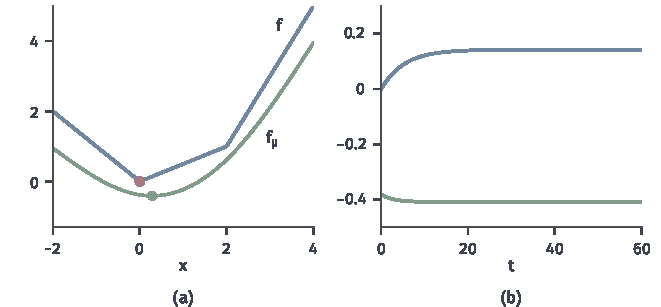
\includegraphics[width=112mm]{figures/05-optimization/03-nonsmooth-optimization/matplotlib/ns-surrogate-rise/figure.pdf}
  \caption{替代目标下降时原目标可以上升。三段折线，$\mu=1$，$\alpha=\tfrac14$，从原问题的解（红点）出发。(a)蓝线是$f$，绿线是$f_\mu$，绿点是$f_\mu$的最小点。(b)蓝线是原目标值，单调上升到平台；绿线是替代目标值，单调下降。}
  \label{fig:ns-surrogate-rise}
\end{BookInlineFigure}

所以光滑化方法要同时记录原目标值，并由式~\eqref{eq:ns-smoothing-split}判断最终结果。这是光滑化与邻近方法的一个重要差别：邻近方法每轮都直接面对原目标$F$。

\section{代理模型}
\label{sec:ns-surrogate}

光滑化一开始就把目标换掉，此后只和替代函数打交道。本节考虑另一种做法：目标不换，每一轮在当前点围绕它造一个容易求解的\term{代理模型}（surrogate model），用模型的解作为候选更新。问题是：模型什么时候能代表原目标取得进展？

模型易解并不说明什么，关键是模型和原目标是什么关系。第~\ref{sec:ns-mm}小节的模型处处在原目标上方，解了就直接下降。第~\ref{sec:ns-bundle}小节的模型处处在下方，只能预测，候选点要回到原目标上检验。

\subsection{MM方法}
\label{sec:ns-mm}

回顾邻近梯度法。式~\eqref{eq:ns-composite-model}的模型在$\alpha\leq1/L$时处处不低于$F$，在当前点与$F$相等，而模型的最小点至少不高于当前值，这三条保证了下降。把这三条抽出来，就不必是二次上界了。

\begin{definition}[上界代理与MM更新]
\label{def:ns-mm}
设$F:\mathbb{R}^n\to\mathbb{R}\cup\{+\infty\}$，$\bm{x}^{(t)}\in\operatorname{dom}F$。函数$Q(\cdot\mid\bm{x}^{(t)})$若满足
\begin{gather}
 Q(\bm{x}\mid\bm{x}^{(t)})\geq F(\bm{x})\qquad\text{对所有}\ \bm{x},\label{eq:ns-mm-majorize}\\
 Q(\bm{x}^{(t)}\mid\bm{x}^{(t)})=F(\bm{x}^{(t)}),\label{eq:ns-mm-touch}
\end{gather}
就称为$F$在$\bm{x}^{(t)}$处的\term{上界代理}（majorizer）。选取满足下式的新点，
\begin{equation}
 Q(\bm{x}^{(t+1)}\mid\bm{x}^{(t)})\leq Q(\bm{x}^{(t)}\mid\bm{x}^{(t)}),
 \label{eq:ns-mm-progress}
\end{equation}
这样的迭代称为\term{MM方法}（majorization-minimization）。
\end{definition}

三项要求合起来给出一串不等式：
\begin{equation}
 F(\bm{x}^{(t+1)})\leq Q(\bm{x}^{(t+1)}\mid\bm{x}^{(t)})\leq Q(\bm{x}^{(t)}\mid\bm{x}^{(t)})=F(\bm{x}^{(t)}).
 \label{eq:ns-mm-chain}
\end{equation}

第一步用上界，第二步用子问题的进展，第三步用接触。所以不需要精确地求最小点，只需要代理值不升。$F$不要求凸，也不要求可微。式~\eqref{eq:ns-mm-chain}的三处都不能少：若只有$\bm{x}^{(t)}$附近上界成立，第一步在远处就失败，候选点要限制在有效区域内；若模型只在当前点相切而不高于$F$，比如凸函数的切线，第一步方向就反了。

可以把上界代理想成在地形上方铺一块柔软的毯子，毯子在脚下贴住地面。把毯子的最低点作为下一步，地面只会比毯子更低，脚下的地面就下降了。

\paragraph{例：绝对值和的二次上界}
要最小化$F(x)=\sum_i\lvert x-y_i\rvert$，也就是求中位数。把每个绝对值换成二次上界。对$c\neq0$，由$(\lvert r\rvert-\lvert c\rvert)^2\geq0$，
\begin{equation}
 \lvert r\rvert\leq\frac{r^2}{2\lvert c\rvert}+\frac{\lvert c\rvert}{2},
 \label{eq:ns-abs-majorizer}
\end{equation}
并且$r=\pm c$时取等号。对每一项取$c=x^{(t)}-y_i$，得到代理
\[
 Q(x\mid x^{(t)})=\sum_i\Bigl(\frac{(x-y_i)^2}{2\lvert x^{(t)}-y_i\rvert}+\frac{\lvert x^{(t)}-y_i\rvert}{2}\Bigr).
\]

代理是二次函数，最小点是加权平均：
\begin{equation}
 x^{(t+1)}=\frac{\sum_iw_iy_i}{\sum_iw_i},\qquad w_i=\frac{1}{\lvert x^{(t)}-y_i\rvert}.
 \label{eq:ns-irls}
\end{equation}

这种由当前残差定权重、解加权最小二乘的方法称为\term{迭代重加权最小二乘}（iteratively reweighted least squares，IRLS）。

用数据$y=(0,1,5)$，从$x^{(0)}=3$开始。此时$F(3)=7$，三个权重是$(\tfrac13,\tfrac12,\tfrac12)$，由式~\eqref{eq:ns-irls}，
\[
 x^{(1)}=\frac{0+\tfrac12+\tfrac52}{\tfrac43}=\frac94,\qquad F(x^{(1)})=6.25.
\]

第二轮的权重变成$(\tfrac49,\tfrac45,\tfrac{4}{11})$，
\[
 x^{(2)}\approx1.628,\qquad F(x^{(2)})\approx5.628.
\]

继续下去依次是$x^{(3)}\approx1.229$和$x^{(4)}\approx1.045$，$F$逐轮降到最优值$5$，最优解是中位数$1$。靠近中位数的数据点权重越来越大，第四轮权重已经约为$22$，这正是非光滑的尖点在代理里的反映。

\begin{BookInlineFigure}
  \centering
  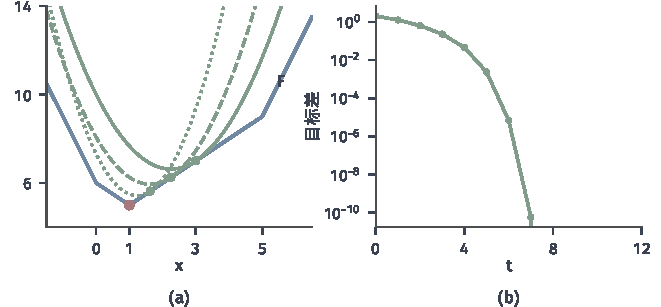
\includegraphics[width=112mm]{figures/05-optimization/03-nonsmooth-optimization/matplotlib/ns-mm-surrogates/figure.pdf}
  \caption{中位数问题的MM迭代，$F(x)=\lvert x\rvert+\lvert x-1\rvert+\lvert x-5\rvert$，$x^{(0)}=3$。(a)蓝线是$F$，绿色实线、虚线、点线是前三轮的二次代理，绿点是接触点，红点是最优解。(b)目标差（对数坐标）逐轮下降。}
  \label{fig:ns-mm-surrogates}
\end{BookInlineFigure}

图~\ref{fig:ns-mm-surrogates}(a)显示每条代理都贴住当前点，并处处在$F$上方。这里也有一个需要小心的地方：当前点若恰好落在某个$y_i$上，$c=0$，式~\eqref{eq:ns-abs-majorizer}没有定义。常用的修正把权重改成$1/\max\{\lvert x^{(t)}-y_i\rvert,\delta\}$。容易误解的是，修正后的代理不再是$\lvert r\rvert$的上界，而是Huber函数$h_\delta(r)$的上界：函数$s\mapsto h_\delta(\sqrt{s})$对$s\geq0$是凹的，取切线就得到这个权重。所以修正后的迭代求解的是第~\ref{sec:ns-huber}小节的替代目标，这时需要按第~\ref{sec:ns-smoothing-accuracy}小节计入偏差。

\paragraph{目标下降与收敛到最优解的区别}
式~\eqref{eq:ns-mm-chain}只说目标值不增。$F$有下界时目标值序列收敛，但它收敛到什么地方，要看$F$本身。

用一个非凸的稀疏罚函数说明。设
\begin{equation}
 F(x)=\frac12(x-3)^2+\frac72\ln(1+\lvert x\rvert).
 \label{eq:ns-reweighted-example}
\end{equation}

函数$s\mapsto\ln(1+s)$在$s\geq0$上是凹的，所以在当前点取切线就是上界。把$\ln(1+\lvert x\rvert)$换成这个上界，代理为
\[
 Q(x\mid c)=\frac12(x-3)^2+\frac72\Bigl(\ln(1+\lvert c\rvert)+\frac{\lvert x\rvert-\lvert c\rvert}{1+\lvert c\rvert}\Bigr).
\]

代理是一个带绝对值的二次函数，最小点由软阈值给出：
\begin{equation}
 x^{(t+1)}=S_{\tau^{(t)}}(3),\qquad\tau^{(t)}=\frac{7/2}{1+\lvert x^{(t)}\rvert}.
 \label{eq:ns-reweighted-update}
\end{equation}

从$x^{(0)}=1$出发，阈值依次是$1.75$，$1.556$，$1.432$，序列是
\[
 1,\ \ 1.25,\ \ 1.444,\ \ 1.568,\ \ldots\to1+\frac{\sqrt2}{2}\approx1.707,
\]
目标值从$4.426$单调下降到约$4.321$。从$x^{(0)}=0.2$出发，阈值是$2.917$，$3.231$，序列是
\[
 0.2,\ \ 0.083,\ \ 0,\ \ 0,\ \ldots
\]
目标值从$4.558$单调下降到$4.5$，然后停住。$x=0$是一个局部最小点：$F$在此处的右导数是$-3+3.5>0$，左导数是$-3-3.5<0$，代理的阈值$3.5$也比数据$3$大。

两条序列都满足不等式链，一条到达全局最优值$4.321$，另一条停在$4.5$。图~\ref{fig:ns-mm-reweighted}显示了这两个吸引域。

\begin{BookInlineFigure}
  \centering
  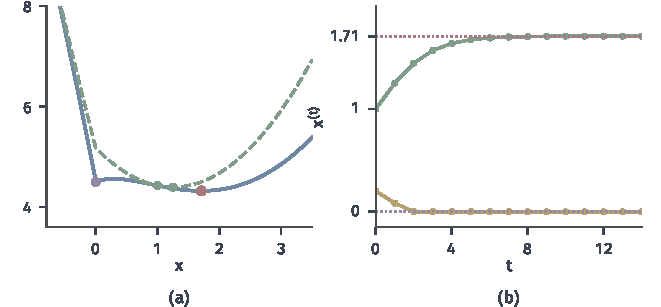
\includegraphics[width=112mm]{figures/05-optimization/03-nonsmooth-optimization/matplotlib/ns-mm-reweighted/figure.pdf}
  \caption{MM在非凸目标上的两个结局，目标是式~\eqref{eq:ns-reweighted-example}。(a)蓝线是$F$，绿色虚线是$x=1$处的代理，绿点是接触点和代理的最小点。红点是全局最优解，紫点是另一个局部最优解$x=0$。(b)迭代序列，绿线从$1$出发到全局最优解，黄线从$0.2$出发停在局部最优解。}
  \label{fig:ns-mm-reweighted}
\end{BookInlineFigure}

要把目标值收敛提升到“极限点是驻点”，还需要额外的条件：常见的要求是代理与原目标在接触点的方向导数一致，代理随当前点连续变化，子问题的解足够接近代理的最小点。要说全局最优，还得有凸性。MM的优点是简单和单调，没有给出离最优值还有多远。

\subsection{束方法}
\label{sec:ns-bundle}

次梯度法每步用一条支撑线，用完就丢了。对凸目标，每一条支撑线都是全局的下界，丢掉很可惜。\term{束方法}（bundle method）把读到的支撑线都留下，拼成一个下界模型。

\paragraph{主要思想}
设$f:\mathbb{R}^n\to\mathbb{R}$是凸函数，读取程序在点$\bm{y}$返回函数值和一个次梯度。假设已经在$\bm{y}^{(0)},\ldots,\bm{y}^{(t)}$处读到次梯度$\bm{g}_0,\ldots,\bm{g}_t$，由支撑不等式，
\begin{equation}
 m^{(t)}(\bm{x})=\max_{0\leq j\leq t}\bigl\{f(\bm{y}^{(j)})+\langle\bm{g}_j,\bm{x}-\bm{y}^{(j)}\rangle\bigr\}\leq f(\bm{x}).
 \label{eq:ns-cutting-plane}
\end{equation}

这个分段线性模型称为\term{割平面模型}（cutting-plane model），读到的这一组支撑线合称束。它在读过的点上等于$f$，别处低估$f$。

直接最小化$m^{(t)}$不行。开始时模型只有一条直线，根本没有最小点；后面它的最小点也可能远远地落在信息不足的地方。解决办法是设一个\term{稳定中心}（stability center）$\hat{\bm{x}}^{(t)}$，表示目前已确认的好点，加一个距离项把候选点拉在中心附近：
\begin{equation}
 \bm{y}^{(t+1)}=\argmin_{\bm{x}}\Bigl\{m^{(t)}(\bm{x})+\frac{1}{2\tau}\lVert\bm{x}-\hat{\bm{x}}^{(t)}\rVert_2^2\Bigr\},\qquad\tau>0.
 \label{eq:ns-bundle-candidate}
\end{equation}

这是模型的邻近映射$\operatorname{prox}_{\tau m^{(t)}}(\hat{\bm{x}}^{(t)})$，解存在且唯一。引入变量$v$表示模型值，子问题是一个小的二次规划：最小化$v+\lVert\bm{x}-\hat{\bm{x}}^{(t)}\rVert_2^2/(2\tau)$，约束是$v$不低于束中每条支撑线在$\bm{x}$处的值。

\paragraph{接受还是拒绝}
模型预测下降
\begin{equation}
 \delta^{(t)}=f(\hat{\bm{x}}^{(t)})-m^{(t)}(\bm{y}^{(t+1)}).
 \label{eq:ns-predicted-decrease}
\end{equation}

因为子问题在$\hat{\bm{x}}^{(t)}$处的值就是$f(\hat{\bm{x}}^{(t)})$（中心处的支撑线在束内），而$\bm{y}^{(t+1)}$是子问题的最小点，所以$\delta^{(t)}\geq0$。但模型是下界，预测往往偏乐观，必须用原目标检验。给定$\beta\in(0,1)$，判断
\begin{equation}
 f(\hat{\bm{x}}^{(t)})-f(\bm{y}^{(t+1)})\geq\beta\,\delta^{(t)}.
 \label{eq:ns-serious-test}
\end{equation}

式~\eqref{eq:ns-serious-test}成立就把中心移到候选点，称为\term{实质步}（serious step）；否则中心不动，称为\term{空步}（null step）。两种情况都把$\bm{y}^{(t+1)}$处的新支撑线加入束。

实质步是有效的移动，空步是对模型的改进。空步没有白费，它恰好在模型低估最严重的地方补上一条割线，下一次预测就准了。这是束方法和前面的方法的一个显著差别：不是每一步都移动，但每一步都学到东西。

\paragraph{计算过程}
用三段折线$f(x)=\max\{-x,x/2,2x-3\}$，$\tau=2$，$\beta=\tfrac12$。

\needspace{6\baselineskip}
\paragraph{变量}
\begin{itemize}
 \item 束：列表$\{(\bm{y}^{(j)},f(\bm{y}^{(j)}),\bm{g}_j)\}$。
 \item $\hat{\bm{x}}^{(t)}$：稳定中心；$\delta^{(t)}$：预测下降。
 \item $\tau$，$\beta$，容差$\varepsilon$。
\end{itemize}

\paragraph{初始化}
选$\bm{y}^{(0)}$，读取$f$和一个次梯度，令$\hat{\bm{x}}^{(0)}=\bm{y}^{(0)}$。例中$y^{(0)}=4$，$f(4)=5$，$g_0=2$。

\needspace{6\baselineskip}
\paragraph{每轮更新}
\begin{enumerate}
 \item 由式~\eqref{eq:ns-bundle-candidate}解候选点。例中第一轮模型只有一条直线，
 \[
  m^{(0)}(x)=2x-3,\qquad y^{(1)}=4-2\tau=0.
 \]
 \item 由式~\eqref{eq:ns-predicted-decrease}算预测下降；若$\delta^{(t)}\leq\varepsilon$，停止，返回$\hat{\bm{x}}^{(t)}$。例中第一轮
 \[
  \delta^{(0)}=5-(-3)=8.
 \]
 \item 读取$f(\bm{y}^{(t+1)})$和次梯度，加入束。例中第一轮
 \[
  f(0)=0,\qquad g_1=\frac12.
 \]
 \item 由式~\eqref{eq:ns-serious-test}决定是否移动中心。例中第一轮实际下降是$5\geq\tfrac12\cdot8$，实质步，中心移到$0$。
\end{enumerate}

第二轮的模型多了一条直线，$m^{(1)}(x)=\max\{2x-3,\ x/2\}$。中心在$0$，子问题的解在$x/2$这一支上，令$\tfrac12+x/2=0$，得到
\[
 y^{(2)}=-1,\qquad m^{(1)}(-1)=-\frac12,\qquad\delta^{(1)}=\frac12.
\]

实际$f(-1)=1$，比中心$f(0)=0$还高，实际下降是$-1$，小于$\beta\delta^{(1)}=\tfrac14$，是空步，中心不动。把$x=-1$处斜率$-1$的支撑线$-x$加入束。

第三轮模型变成$\max\{2x-3,\ x/2,\ -x\}$，在中心$0$的次微分是$[-1,\tfrac12]$，包含$0$，所以$y^{(3)}=0$，
\[
 \delta^{(2)}=0.
\]

预测下降为零，停止，最终得到$\hat{x}=0$，也就是最优解。图~\ref{fig:ns-bundle-1d}逐轮画出了模型：(b)的模型过分乐观，(c)补上割线后预测就准了。

\begin{BookInlineFigure}
  \centering
  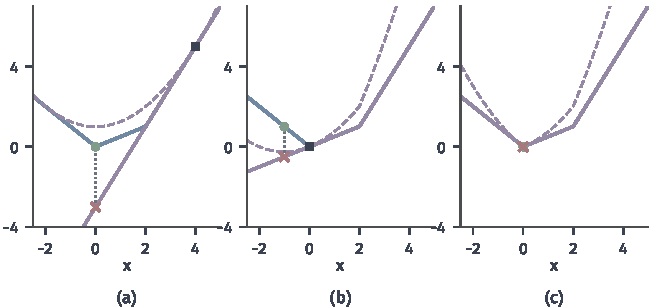
\includegraphics[width=112mm]{figures/05-optimization/03-nonsmooth-optimization/matplotlib/ns-bundle-1d/figure.pdf}
  \caption{束方法在三段折线上的三轮，$\tau=2$。蓝线是$f$，紫色实线是割平面模型，紫色虚线是模型加距离项，黑方块是稳定中心。红叉是候选点处的模型值，绿点是候选点处的真实目标值。(a)第一轮，实质步。(b)第二轮，候选点$-1$处模型偏低，真实目标值反而高，空步。(c)第三轮，候选点就是中心，预测下降为零，停止。}
  \label{fig:ns-bundle-1d}
\end{BookInlineFigure}

\paragraph{评价原目标的误差}
预测下降$\delta^{(t)}$既用于接受判断，也是一个停止证书。子问题的最优性条件给出
\[
 \bm{s}^{(t)}=\frac{\hat{\bm{x}}^{(t)}-\bm{y}^{(t+1)}}{\tau}\in\partial m^{(t)}(\bm{y}^{(t+1)}).
\]

由模型是$f$的下界和$\bm{s}^{(t)}$是模型的次梯度，对任意$\bm{x}$，
\[
 f(\bm{x})\geq m^{(t)}(\bm{x})\geq m^{(t)}(\bm{y}^{(t+1)})+\langle\bm{s}^{(t)},\bm{x}-\bm{y}^{(t+1)}\rangle.
\]

由式~\eqref{eq:ns-predicted-decrease}替换模型值，再用$\bm{s}^{(t)}$的定义把候选点写成$\hat{\bm{x}}^{(t)}$减$\tau\bm{s}^{(t)}$，整理后得到
\begin{equation}
 f(\bm{x})\geq f(\hat{\bm{x}}^{(t)})+\langle\bm{s}^{(t)},\bm{x}-\hat{\bm{x}}^{(t)}\rangle-e^{(t)},\qquad e^{(t)}=\delta^{(t)}-\tau\lVert\bm{s}^{(t)}\rVert_2^2.
 \label{eq:ns-bundle-certificate}
\end{equation}

取$\bm{x}=\hat{\bm{x}}^{(t)}$得$e^{(t)}\geq0$，所以$\tau\lVert\bm{s}^{(t)}\rVert_2^2\leq\delta^{(t)}$，$e^{(t)}\leq\delta^{(t)}$。式~\eqref{eq:ns-bundle-certificate}说$\bm{s}^{(t)}$是一个带误差$e^{(t)}$的近似次梯度。设中心到某个最优解的距离不超过$R$，在式中取$\bm{x}=\bm{x}^\star$，得到
\begin{equation}
 f(\hat{\bm{x}}^{(t)})-f^\star\leq e^{(t)}+R\lVert\bm{s}^{(t)}\rVert_2\leq\delta^{(t)}+R\sqrt{\frac{\delta^{(t)}}{\tau}}.
 \label{eq:ns-bundle-error}
\end{equation}

这个界每一轮都可以直接计算，不需要任何收敛定理。例中第三轮$\delta^{(2)}=0$，$\bm{s}^{(2)}=0$，这一轮的证书说明误差为零。

\paragraph{收敛与成本}
在凸目标、次梯度有界的条件下，邻近束方法的中心目标值收敛到$f^\star$，实质步无穷多和有限多两种情形要分别讨论，证明篇幅较长。这里强调它的成本结构。

图~\ref{fig:ns-bundle-2d}在平面上比较束方法与次梯度法，横轴是原目标的读取次数。束方法只用很少几次读取就到达很高的精度，这得益于分段线性目标正好是割平面模型的同类，代价是每轮要解一个二次规划，约束个数随束增长。实践中会合并或丢弃不活跃的割线，这需要额外的规则来保证模型仍然有效。

\begin{BookInlineFigure}
  \centering
  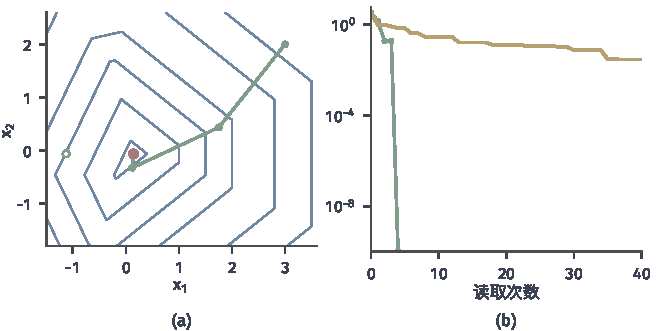
\includegraphics[width=112mm]{figures/05-optimization/03-nonsmooth-optimization/matplotlib/ns-bundle-2d/figure.pdf}
  \caption{束方法与次梯度法，目标与图~\ref{fig:ns-smoothing-budget}相同，$\bm{x}^{(0)}=(3,2)$。(a)蓝线是等高线，红点是最优解，绿色实心点和折线是实质步，空心圆是空步的候选点。(b)绿线是束方法的中心目标差，黄线是次梯度法的最好目标差（步长$\sqrt{13}/\sqrt{t+1}$），横轴是原函数读取次数，纵轴为对数坐标。}
  \label{fig:ns-bundle-2d}
\end{BookInlineFigure}

\paragraph{上界模型与下界模型}
两种模型提供的信息不同，表~\ref{tab:ns-surrogates}把它们和前面的光滑化放在一起比较。上界模型给出保证而无需再读原目标，但不告诉离最优有多远。下界模型给出离最优的证书，但每步都要检验。把下界模型的解直接当作进展，或者把上界模型的最小值当作下界，都是错误的用法。

\begin{BookInlineTable}
  \centering
  \small
  \begin{tabular}{@{}llll@{}}
    \toprule
     & MM & 束方法 & 光滑化\\
    \midrule
    辅助函数 & 上界，每轮重建 & 下界，逐轮累加 & 固定的光滑替代\\
    与原目标的关系 & 处处在上方 & 处处在下方 & 相差不超过$\mu D$\\
    接受规则 & 代理值不增 & 实际下降够大 & 无\\
    原目标逐轮 & 不增 & 中心不增 & 可以上升\\
    误差证书 & 无 & 式~\eqref{eq:ns-bundle-error} & 式~\eqref{eq:ns-smoothing-split}\\
    主要成本 & 代理子问题 & 二次规划 & 梯度次数\\
    \bottomrule
  \end{tabular}
  \caption{三种辅助模型的对照。}
  \label{tab:ns-surrogates}
\end{BookInlineTable}

\section{本章小结}
\label{sec:ns-summary}

本章从一个具体的麻烦开始：Lasso的解恰好落在目标不可微的地方。为此先用支撑直线的斜率定义了次梯度和次微分，凸目标的最优解由$\bm{0}\in\partial f$充要地刻画；和与复合的规则需要相对内部这样的正则条件。非凸函数上要改用局部定义的广义导数，那时的条件只是必要的。

此后各节回答“用什么信息推进迭代”，答案不同，要求和保证也不同。

次梯度法只用支撑信息，每步一个次梯度，单步不一定下降，但距离的递推使平均点或最好点的目标差为$O(1/\sqrt{T})$，这在黑箱模型下不能本质改进。

邻近方法把难求导的结构留在子问题里。复合目标的邻近梯度法（ISTA）在凸情形达到$O(1/T)$，FISTA用外推达到$O(1/T^2)$，后者不要求逐轮下降，也不能直接用于非凸目标；非凸情形用映射残差评价，残差为零只说明是复合驻点。邻近方法的前提是邻近映射可算，映射可定义、子问题可计算和原问题收敛是三件要分别核对的事。

光滑化和代理模型改变每一步要解的问题。Huber函数是绝对值的Moreau包络，Nesterov平滑利用最大值结构在内层加强凸项，它们用偏差$\mu D$换取$O(1/\mu)$的光滑常数，原目标的误差由偏差和求解误差两部分决定；平滑改变目标，加速改变迭代规则，配合使用可得$O(1/\varepsilon)$的总步数。MM用上界代理保证原目标不增，束方法用支撑线拼成的下界模型预测下降，并用接受规则和预测下降值来评价真实进展。

\begin{BookInlineTable}
  \centering
  \small
  \begin{tabular}{@{}lll@{}}
    \toprule
    方法 & 需要的结构 & 凸情形的保证\\
    \midrule
    次梯度法 & 次梯度有界 & 目标差$O(1/\sqrt{T})$\\
    邻近点法 & $\operatorname{prox}_{\alpha f}$可算 & 目标差$O(1/\sum\alpha^{(t)})$\\
    ISTA & $\nabla f$，$\operatorname{prox}_{\alpha r}$ & 目标差$O(1/T)$，单调\\
    FISTA & 同上 & 目标差$O(1/T^2)$，不单调\\
    平滑加速 & 最大值结构，内层可解 & $O(1/\varepsilon)$步，带偏差$\mu D$\\
    MM & 上界代理 & 目标值不增\\
    束方法 & 次梯度，二次规划求解 & 可计算的误差证书\\
    \bottomrule
  \end{tabular}
  \caption{本章方法的对照。$T$为迭代步数，$\varepsilon$为原目标精度。}
  \label{tab:ns-summary}
\end{BookInlineTable}

表~\ref{tab:ns-summary}把这些方法放在一起。本章全部在无约束或简单约束下讨论，一般约束的乘子、增广Lagrange函数与ADMM由第~\ref{chap:penalty-multiplier-methods}章结合约束结构建立；按变量分块使用邻近映射的方法见第~\ref{chap:block-optimization}章。


